\section{TSP团队软件过程}
TSP提供了
\vspace{-0.8em}
\begin{multicols}{3}
    \begin{itemize}
        \item 一个已定义的团队构建过程
        \item 一个团队作业框架
        \item 一个有效的管理环境
    \end{itemize}
\end{multicols}
\vspace{-1em}

\subsection{团队工程开发:需求开发}
需求开发包含需求获取、需求汇总、需求验证

\subsubsection{需求分类}
\textbf{客户需求}描述的是客户的期望,是客户解决问题的愿望
\begin{itemize}
    \item 客户需求可能很简单,也可能很复杂;可能很清晰,也可能模糊
    \item 比如,客户希望有一种快速进行数据计算的工具帮助其完成繁琐的计算工作
\end{itemize}

\textbf{产品需求}描述的是开发团队所提供的解决方案。即针对上述的客户需求,开发团队设计出一个可以帮助客户解决工作当中碰到的问题的方案。

\textbf{产品组件}需求描述的是组成产品的各个组件的需求规格。与产品需求相比,这是更低层次,更为细致的描述了上述解决方案中的某个组件的功能、性能与形式等。

\subsubsection{为什么说“需求是一切工程活动的基础”}
\begin{itemize}
    \item 设计活动一定是依据需求而开展的
    \item 产品集成活动中,各个组件之间的接口必须满足事先确定的接口需求,否则会造成接口不匹配
    \begin{itemize}
        \item 验证(Verification)活动也是检验获得的产品和产品组件能不能满足各自事先定义好的需求规格
        \item 确认(Validation)活动是为了确保产品可以满足客户的需求以及实际操作场景的要求
    \end{itemize}
    \item 此外,需求也是项目计划活动的关键输入。比如,项目的规模估算、成本估算等必须参考需求来进行
\end{itemize}

\subsubsection{需求获取}
需求是采用“诱导”式方法获取客户的显式需求和隐式需求,尽可能的识别客户的期望与所受到的限制
\begin{itemize}
    \item “诱导”不仅仅是普通的需求采集,隐含了更加积极地、前瞻性地识别那些客户没有明确提供的额外需求
    \item 客户所受到的限制也应当作为需求开发过后需要关注的内容。限制包括技术、成本、时间、风险、行业规则、法律等等
\end{itemize}

\subsubsection{需求汇总}
\begin{itemize}
    \item 整理各种来源的信息,识别缺失的信息
    \item 解决冲突的需求
    \begin{itemize}
        \item 需求的整理和转化:我们需要将客户的需求转换为产品需求和产品组件的需求
        \item 推导未显式描述的需求内容,例如采用某项技术的附属需求
    \end{itemize}
\end{itemize}

\subsubsection{需求验证}
对需求进行分析和确认,以确保符合使用者预期,典型活动包括:
\begin{itemize}
    \item 建立和维护操作概念和相关的场景;场景一般而言是指使用产品时可能发生的时间顺序
    \item 分析需求,以确保其必要性、充分性和平衡性
    \item 确认需求,以确保将要产生的产品能在预期的用户环境中运行并且工作正常
\end{itemize}

\subsubsection{需求文档制作}
需求开发工作完成的一个基本标志是形成了一份完整的、规范的、经过评审的需求规格说明书

需求规格说明书的编制是为了使用户和软件开发者双方对该软件的初始规定有一个共同的理解,使之成为整个开发工作的基础

\paragraph{优秀需求规格文档特征}~{} \par
\vspace{-0.5em}
\begin{spacing}{1.2}
    \centering
    \begin{longtable}{|m{2cm}<{\centering}|m{13cm}|}
        \hline
        \textbf{特征} & \multicolumn{1}{c|}{\textbf{描述}}                                                         \\ \hline
        内聚特征        & 需求规格描述应当尽可能内聚,即仅仅用以说明一件事情                                                                \\ \hline
        完整特征        & 需求规格描述应当完整,不能遗漏信息                                                                        \\ \hline
        一致特征        & 需求规格描述的各个条目和章节不能互相矛盾,需求规格描述与所有外部的参考资料之间也应当消除矛盾之处                                         \\ \hline
        原子特征        & 需求规格描述的过程中,应当尽可能避免连接词的使用。如果需要描述多项内容,可以分别用简单语句加以描述                                        \\ \hline
        可跟踪特征       & 客户需求、产品需求以及产品组件需求必须可以双向跟踪,即客户需求的任何内容,都应当在产品需求和产品组件需求中得到体现。反之,产品组件需求的每一项描述也要可以跟踪到客户需求中的内容 \\ \hline
        非过期特征       & 需求描述的内容必须体现相关干系人对于项目的最新认识。即不能包含已经废弃的需求定义                                                 \\ \hline
        可行性特征       & 需求规格描述的各项内容应该在项目所拥有的资源范围内可以实现                                                            \\ \hline
        强制特征        & 需求规格描述的内容应当体现强制性,即需求规格描述的内容的任何一项缺失,都会导致最终产品不能满足客户期望。因此,可选的需求内容要么不要出现,要么以明确的方式标注          \\ \hline
        可验证特征       & 需求规格描述应当便于在后期开发过程中进行验证。即实现该需求与否,应该有明确的判断标准                                               \\ \hline
    \end{longtable}
\end{spacing}
\vspace{-1em}

\paragraph{SRS示例}~{} \par
\vspace{-0.8em}
\begin{multicols}{5}
    \begin{enumerate}[label=\arabic*.]
        \item 引言
        \item 系统定义
        \item 应用环境
        \item 功能规格
        \item 性能需求
        \item 实现约束
        \item 质量描述
        \item 其它要求
        \item 参考材料
        \item 签字认证
    \end{enumerate}
\end{multicols}
\vspace{-1em}

对于需求规格模板中的功能规格定义可以用多种方式灵活定义。典型的方式有原型描述、结构化分析方法描述、用例描述、可测试需求列表描述等

\subsubsection{考试题目}
\begin{problem}
请解释需求开发中客户需求和产品需求的差别,并设计一个流程来完成需求开发工作
\end{problem}

\begin{problem}
请给出需求开发的完整过程,并且解释客户需求和产品需求的各自含义以及在需求开发过程中该如何体现客户需求和产品需求
\end{problem}

\subsection{团队工程开发:团队设计}

\subsubsection{团队智慧}
发挥团队智慧两大挑战:
\vspace{-0.8em}
\begin{multicols}{2}
    \begin{itemize}
        \item 确定整体架构之前很难进行分工
        \item 鼓励团队成员在讨论和评审会议中的参与程度
    \end{itemize}
\end{multicols}
\vspace{-1em}

\subsubsection{设计标准}
\begin{itemize}
    \item 命名规范:项目小组应当设计一个统一的命名规范来命名各个模块并建立系统词典
    \item 接口标准:组件之间的接口标准和格式也需要作为设计标准的内容之一加以定义
    \item 系统出错信息:系统异常信息和出错信息往往也需要通过一个规范加以标准化
    \item 设计表示标准:设计表示标准定义了设计工作的产物应当满足的标准
\end{itemize}

\subsubsection{复用性支持}
在设计阶段必须要充分考虑复用的可能。为了支持复用,软件项目团队需要建立一套复用管理流程,具体而言,包括:
\vspace{-0.8em}
\begin{multicols}{3}
    \begin{itemize}
        \item 复用接口标准
        \item 复用文档标准
        \item 复用质量保证机制
    \end{itemize}
\end{multicols}
\vspace{-1em}

\subsubsection{可测试性考虑}
设计可测试性考虑主要体现在两方面:
\vspace{-0.8em}
\begin{multicols}{2}
    \begin{itemize}
        \item 要尽可能减少测试代码的数量
        \item 要制作合理的测试计划
    \end{itemize}
\end{multicols}
\vspace{-1em}

\subsubsection{可用性考虑}
\begin{itemize}
    \item 可用性的问题应当在设计阶段就开始考虑,而不能推延到实现阶段
    \item 针对每一个关键功能都定义操作概念和操作场景
    \item 分析操作场景以确保软件系统开发完成之后,系统使用者会满意
    \item 必要时,可以邀请最终用户参与场景的评审,使用模拟、原型等技术,更好的把握用户真实意图
\end{itemize}

\subsubsection{设计的文档化}
\vspace{-0.8em}
\begin{multicols}{3}
    \begin{enumerate}[label=\arabic*.]
        \item 引言
        \item 设计文档目的
        \item 问题陈述
        \item 团队信息
        \item 高层设计
        \begin{enumerate}[label=\alph*.]
            \item 系统架构
            \item 组件分配表
            \item 功能规格说明
            \item 操作场景
            \item 各个模块工作方式的伪码描述
            \item 用户界面
        \end{enumerate}
        \item 详细设计
        \begin{enumerate}[label=\alph*.]
            \item 状态机设计
            \item 模块内部工作方式的伪码描述   
        \end{enumerate}
        \item 限制条件
        \begin{enumerate}[label=\alph*.]
            \item 标准兼容
            \item 硬件限制
            \item 开发限制   
        \end{enumerate}
        \item 参考材料
    \end{enumerate}
\end{multicols}
\vspace{-1em}

\subsection{团队工程开发:实现策略}

\subsubsection{评审的考虑}
\begin{itemize}
    \item 设计的时候采用的策略是自顶向下、逐层精化,这有利于建立系统的整体观
    \item 实现的时候为了方便对实现结果评审,建议采用自底向上的方式进行,首先实现底层的内容,然后对这些底层的模块进行评审,有利于复用策略的应用
\end{itemize}

\subsubsection{复用策略}
采用自底向上的开发策略有利于进行复用,几个经典的复用策略:
\begin{itemize}
    \item \textbf{编码注释的应用}:编码注释采用统一格式,标明功能,调用方式。异常信息等有利于复用的信息
    \item \textbf{站立式会议}:在会上,团队成员可以讨论实现计划,识别可复用组件,了解现有的复用组件库的内容
\end{itemize}

\subsubsection{可测试性考虑}
实现计划必须与测试计划一致,不能出现集体测试的时候部分模块未实现的情况

\subsection{团队工程开发:集成策略选择}
\vspace{-0.5em}
\begin{spacing}{1.2}
    \centering
    \begin{longtable}{|m{2cm}<{\centering}|m{4.1cm}|m{4.1cm}|m{4.1cm}|}
        \hline
        \textbf{策略名} & \multicolumn{1}{c|}{\textbf{特点}}                               & \multicolumn{1}{c|}{\textbf{优点}}            & \multicolumn{1}{c|}{\textbf{缺点}}                                   \\ \hline
        大爆炸集成策略      & 将所有已经完成的组件放在一起进行一次集成                                           & 需要很少的测试用例                                   & 需要所有有待集成的组件质量非常高,否则会出现难以定位缺陷位置的问题,从而消耗很多测试时间;另外,系统越复杂,规模越大,问题越突出   \\ \hline
        逐一添加集成策略     & 与大爆炸集成策略相反,采取一次添加一个组件的方式进行集成                                   & 很容易定位缺陷位置,特别是在产品组件质量不高的情况下,每次集成之前都有着坚实的质量基础 & 需要测试用例非常多;存在有大量的回归测试,测试时间成本大                                       \\ \hline
        集簇集成策略       & 是对逐一添加集成策略的改进,把有相似功能或者有关联的模块优先进行集成,形成可以工作的组件,然后以组件为单位继续较高层次的集成 & 可以尽早获得一些可以工作的组件,有利于其它组件测试工作的开展              & 过于关注个别组件,而缺乏系统的整体观,不能尽早发现系统层面的缺陷                                   \\ \hline
        扁平化集成策略      & 优先集成高层的部件,然后逐步将各个组件、模块的真正实现加入系统。即尽快构建一个可以工作的扁平化系统              & 可以尽早发现系统层面的缺陷                               & 为了确保完成的系统,需要大量的打“桩”(stub),即提供一些直接提供返回值的伪实现。这种方式往往不能覆盖整个系统应该处理的多种状态 \\ \hline
    \end{longtable}
\end{spacing}
\vspace{-1em}


\subsubsection{考试题目}
\begin{problem}
产品组件集成策略有哪些?请解释这些策略的优缺点。在此基础上,解释如果要实现高质量集成,可能需要注意哪些方面。
\end{problem}

\begin{problem}
请罗列集成测试的典型策略,并且解释各个集成测试策略的优缺点?
\end{problem}

\subsection{团队工程开发:验证与确认V\&V}

\subsubsection{什么是V\&V}
\begin{itemize}
    \item 验证(Verification)活动也是检验获得的产品和产品组件能不能满足各自事先定义好的需求规格
    \item 确认(Validation)活动是为了确保产品可以满足客户的需求以及实际操作场景的要求
    \item 验证(Verification)和确认(Validation)都是为了提升最终产品的质量而采取的措施
\end{itemize}

\subsubsection{V\&V的区别与联系}
验证和确认的目的不同:
\begin{itemize}
    \item 验证是目的是确保选定的工作产品与事先指定给该工作产品的需求(即产品需求或产品组件需求)一致
    \item 确认的目的则是确保开发完成的产品或者产品组件在即将要使用该产品或者产品组件的环境中工作正确,关注的是客户需求的满足
\end{itemize}

验证和确认又是相互依存、关系紧密的两个活动
\begin{itemize}
    \item 验证活动的依据来源于确认的目标,即产品组件需求必须与客户需求一致
    \item 验证活动为确认活动提供了前提条件,在完成产品需求和产品组件需求之前,考虑客户需求是否满足是没有意义的
\end{itemize}

\subsubsection{V\&V的活动}
\vspace{-0.5em}
\begin{spacing}{1.2}
    \centering
    \begin{longtable}{|m{1.5cm}<{\centering}|m{13.8cm}|}
        \hline
        \textbf{活动} & \multicolumn{1}{c|}{\textbf{说明}} \\ \hline
        环境准备 & 
        \vspace{-1.1em}
        \begin{enumerate}[label=,leftmargin=0em]
            \item 对于验证工作,如果是评审,则需要准备文件材料、人员以及会议场所等;如果是测试,需要准备模拟器、场景生成程序、环境控制以及其他系统接口等
            \item 对于确认工作,则需要模拟真实环境和场景
        \vspace{-1.3em}
        \end{enumerate}
        \\ \hline
        对象选择 & 
        \vspace{-1.1em}
        \begin{enumerate}[label=,leftmargin=0em]
            \item 对于验证工作,验证对象往往从工作产品中选择
            \item 对于确认工作,确认对象从产品中选择
        \vspace{-1.3em}
        \end{enumerate}
        \\ \hline
        活动实施 & 
        \vspace{-1.1em}
        \begin{enumerate}[label=,leftmargin=0em]
            \item 确认工作活动包括早期对产品需求评审工作和最后的验收测试
            \item 验证工作:一般的评审和测试工作
        \vspace{-1.3em}
        \end{enumerate}
        \\ \hline
        结果分析 &
        \vspace{-1.1em}
        \begin{enumerate}[label=,leftmargin=0em]
            \item 对于评审结果,可以根据评审结果反思软件开发过程的合理性、以及是否还有隐藏的缺陷
            \item 对于验收测试的结果,则可以关注那些一直遗留到验收阶段才被发现的缺陷,看看这些缺陷在什么阶段被引入,为什么前面未能发现等
        \vspace{-1.3em}
        \end{enumerate} 
        \\ \hline
    \end{longtable}
\end{spacing}
\vspace{-1em}


\subsubsection{V\&V的例子}
\vspace{-0.8em}
\begin{multicols}{4}
    \begin{itemize}
        \item 单元测试:验证
        \item 集成:验证
        \item 需求评审:确认
        \item 验收测试:确认
    \end{itemize}
\end{multicols}
\vspace{-1em}

\subsubsection{考试题目}
\begin{problem}
请解释在质量保障活动中的V\&V分别是什么含义?两者之间的关系是什么?
\end{problem}

\begin{problem}
请举例说明验证和确认的区别和联系? 
\end{problem}

\subsection{团队项目规划:工作分解结构与范围管理}

\subsubsection{工作分解结构}
工作分解结构(WBS, Work Breakdown Structure)是以可交付成果为导向对满足项目目标和开发交付产物的项目相关工作进行的分解
\vspace{-0.8em}
\begin{multicols}{2}
    \begin{itemize}
        \item 它归纳和定义了项目的整个工作范围
        \item 每下降一层代表对项目工作的更详细定义
    \end{itemize}
\end{multicols}
\vspace{-1em}

作用/特点:
\begin{itemize}
    \item 提供了\textbf{项目范围基线},是范围变更的重要输入
    \item 可以展现\textbf{项目整体观},使得项目团队成员可以集中注意力实现项目的目标上
    \item 为开发项目提供了一个整体框架,\textbf{防止遗漏}项目的可交付成果
    \item 使得项目中各个角色的责任更明确,帮助项目团队的建立和获得项目成员的承诺
    \item 为评估和分配任务提供具体的工作包的定义,工作包可以分配给项目某个成员或者另一个团队
    \item 是进行估算和编制项目日程计划的基础
    \item 可以帮助项目团队理解工作内容,分析项目的风险
\end{itemize}

表示方式:树型层次结构;清单型层次结构

\paragraph{创建WBS}~{} \par
将复杂的项目逐步分解为一系列明确定义的工作任务并作为随后计划活动的指导文档

要将整个项目分解成工作包:
\vspace{-0.8em}
\begin{multicols}{2}
    \begin{enumerate}[label=\arabic*.]
        \item 识别和分析可交付成果以及相关工作
        \item 确定工作分解结构的结构与编排方法
        \item 自上而下逐层细化分解
        \item 为工作分解结构组成部分制定和分配标志编码
        \item 核实工作分解的程度是必要且充分的
    \end{enumerate}
\end{multicols}
\vspace{-1em}

\paragraph{好的WBS的检查标准}~{} \par
\begin{itemize}
    \item 最底层要素不能重复,即任何一个工作应该在WBS中的一个地方且只应该在WBS中的一个地方出现
    \item 所有要素必须清晰完整定义,即相应的数据词典必须完整定义
    \item 最底层要素必须有定义清晰的责任人,可以支持成本估算和进度安排
    \item 最底层要素是实现目标的成分必要条件,即项目的工作范围得到完整体现
\end{itemize}

\subsubsection{范围管理}
包括确保项目做且只做成功完成项目所需的全部工作的各过程,WBS为范围管理提供了基础:
\vspace{-0.8em}
\begin{multicols}{5}
    \begin{itemize}
        \item 收集需求
        \item 定义范围
        \item 创建WBS
        \item 核实范围
        \item 控制范围变更
    \end{itemize}
\end{multicols}
\vspace{-1em}

\subsection{团队项目规划:开发策略与计划}
定义:是在产品组件需求基础之上,明确每个产品组件的获得方式与顺序,从而在项目团队内部建立起大家都理解的产品开发策略

注意事项:
\vspace{-0.8em}
\begin{multicols}{3}
    \begin{itemize}
        \item WBS的使用
        \item 产品组件开发顺序的考虑
        \item 产品组件获得方式的考虑
    \end{itemize}
\end{multicols}
\vspace{-1em}

\subsection{团队项目规划:生命周期模型选择}
\begin{wraptable}{r}{0.4\textwidth}
    \centering
    \vspace{-4.5em}
    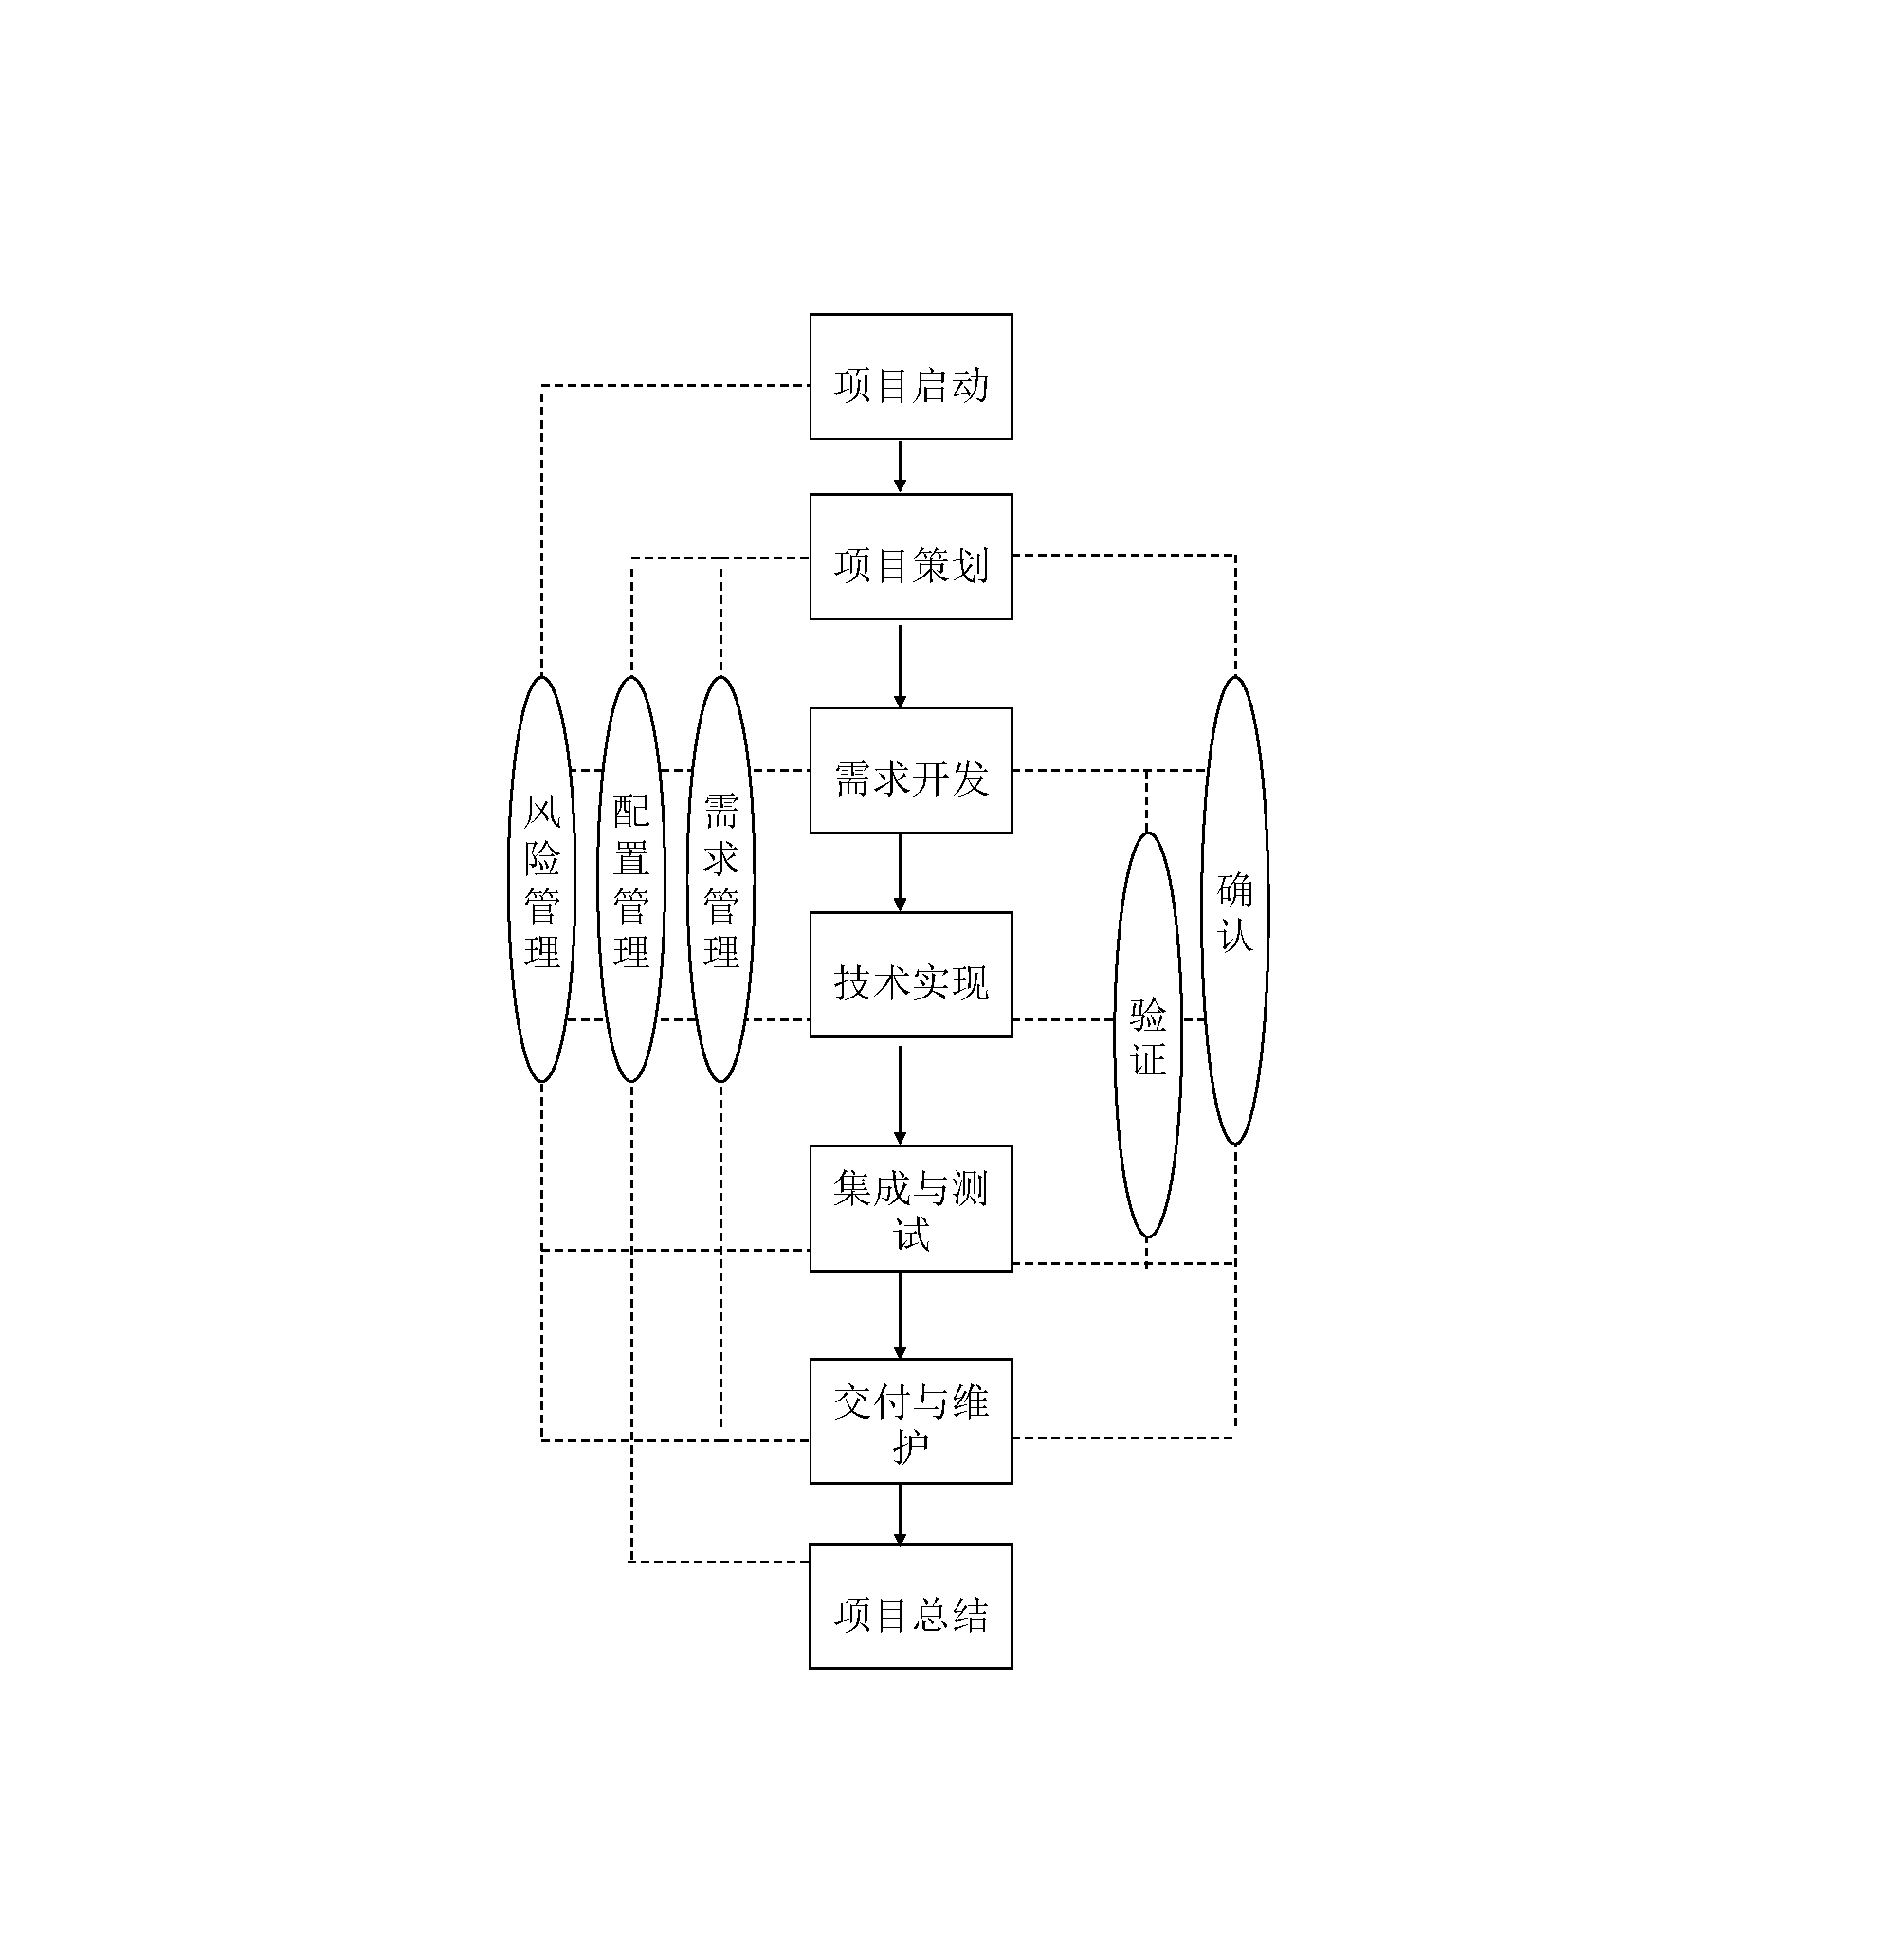
\includegraphics[width=0.32\textwidth]{images/生命周期模型.pdf}
    \vspace{-10.5em}
\end{wraptable}
生命周期模型的各个阶段
\begin{itemize}
    \item 项目启动阶段
    \item 项目策划阶段
    \item 需求开发阶段
    \item 技术实现阶段
    \item 集成与测试阶段
    \item 交付与维护阶段
    \item 项目总结
\end{itemize}

\subsection{团队项目规划:计划}

\subsubsection{日程计划原理和方法}
\paragraph{任务计划和日程计划}~{} \par
\begin{itemize}
    \item \textbf{任务计划}描述了项目所有的任务清单,任务之间的先后顺序以及每个任务所需时间资源
    \item \textbf{日程计划}描述了每个任务在日志上的安排,即每个任务计划哪天开始和计划哪天结束
    \item 制定资源计划,结合任务计划就可以定义日程计划
    \item 团队形式的日程计划考虑:
    \begin{itemize}
        \item 资源平衡:要求项目团队结合每个团队成员的工作效率、工作内容以及资源水平,找到一个时间点,让所有团队成员几乎同时完成任务
        \item 资源同步:安排日程时必须兼顾某些项目人物之间的依赖关系
    \end{itemize}
\end{itemize}

\paragraph{典型计划流程回顾}~{} \par
\vspace{-0.8em}
\begin{multicols}{3}
    \begin{itemize}
        \item 估算规模
        \item 估算资源
        \item 规划日程
    \end{itemize}
\end{multicols}
\vspace{-1em}

\subsubsection{质量计划原理和方法}
\begin{wraptable}{r}{0.55\textwidth}
    \centering
    \vspace{-4.3em}
    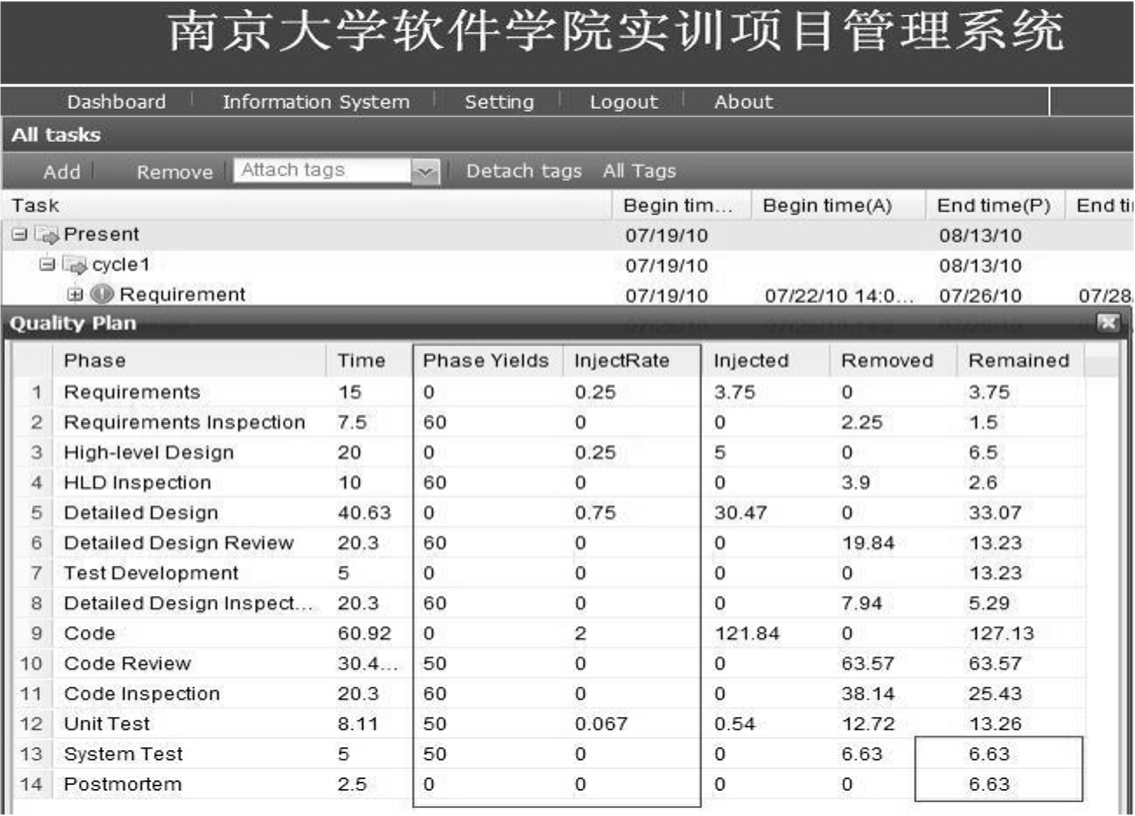
\includegraphics[width=0.55\textwidth]{images/质量计划原理和方法.png}
    \vspace{-10.5em}
\end{wraptable}
项目的质量计划中应当确定需要开展的质量保证活动
\begin{itemize}
    \item 典型的质量保证活动包括了个人评审、团队评审、单元测试、集成测试以及验收测试等
    \item 在质量计划中需要解决的关键问题是该开展哪些活动,以及这些活动开展的程度,如时间、人数和目标是什么
\end{itemize}

\subsubsection{风险计划}
风险管理的\textbf{目标}是:在风险发生前,识别出潜在的问题,以便在产品或项目的生命周期中规划和实施风险管理活动,以消除潜在问题对项目产生的负面影响

风险管理是一个持续的、前瞻的过程,此过程是项目管理的重要部分。有效的风险管理是通过相关干系人的合作与参与,尽快且积极地识别风险,指定项目风险管理计划
\begin{itemize}
    \item 风险管理需要同时考虑有关成本、进度、绩效以及其他风险的内部及外部来源
    \item 在项目初期进行变更或修正的工作负荷,通常比在项目后期来得容易、花费较低且较不具破坏性
    \item 早期且积极的风险侦测是重要的
\end{itemize}

风险管理大致分为两部分,即\textbf{风险识别}和\textbf{风险应对}

早期风险侦测的重要性:在项目初期进行变更或修正的工作负荷,通常比在项目后期来得容易、花费较低及较不具破坏性

\paragraph{风险识别}~{} \par
\begin{itemize}
    \item 风险:没有发生,有一定概率会发生,发生后有一定影响
    \item 问题:已经发生的,比如人员调动等
\end{itemize}

典型的识别方法:
\vspace{-0.8em}
\begin{multicols}{2}
    \begin{enumerate}[label=\arabic*.]
        \item 检查WBS的每个组件以找出相应的风险
        \item 使用定义好的风险分类表上来评估风险
        \item 访谈相关的领域专家
        \item 与类似项目进行比较来审查风险管理
        \item 检查以往项目的总结报告或组织级数据库
        \item 检查设计规格和协议书需求
    \end{enumerate}
\end{multicols}
\vspace{-1em}

典型的风险识别活动包括:
\vspace{-0.8em}
\begin{multicols}{2}
    \begin{enumerate}[label=\arabic*.]
        \item 识别与成本、进度及绩效相关的风险
        \item 审查可能影响项目的环境因素
        \item 审查工作分解结构的所有组件,作为风险识别的一部分,以协助确保所有的工作投入均已考虑
        \item 审查项目计划的所有组件,作为风险识别的一部分,以确保项目在各方面均已考虑
        \item 记录风险的内容、条件及可能的结果
        \item 识别每一风险相关的干系人
        \item 利用已定义的风险参数,评估已识别的风险
        \item 依照定义的风险类别,将风险分类并分组
        \begin{itemize}
            \item 可能性很低,但是发生影响程度很大:政策变化、领导层大规模变动、公司倒闭
            \item $[P\mbox{(可能性)}, I\mbox{(影响程度)}, T\mbox{(阈值)}]$
        \end{itemize}
    \end{enumerate}
\end{multicols}
\vspace{-1em}

\paragraph{风险应对}~{} \par
识别风险之后,就应当制定相应的风险管理策略,以应对各类风险

典型的策略包括:
\vspace{-0.5em}
\begin{spacing}{1.2}
    \centering
    \begin{longtable}{|m{2cm}<{\centering}|m{13cm}|}
        \hline
        \textbf{策略} & \multicolumn{1}{c|}{\textbf{特点}} \\ \hline
        风险转嫁 &
        \vspace{-1.1em}
        \begin{enumerate}[label=,leftmargin=0em]
            \item 指通过某种安排,在放弃部分利益的同时,将部分的项目风险转嫁到其他的团队或者组织
            \item 比如有的公司采取外包的方式,把一部分有技术风险的产品组建交由其他公司开发,在放弃部分收益的同时,也规避了技术风险
            \vspace{-1.1em}
        \end{enumerate}
        \\ \hline
        风险解决 &
        \vspace{-1.1em}
        \begin{enumerate}[label=,leftmargin=0em]
            \item 指采用一些有效措施,使得风险的来源不再存在
            \item 这往往是一种预防性的手段,比如针对项目面临的技术风险,采取技术调研或者引进技术专家的手段,使得原有的风险来源不再存在或者存在可能性极低,从而测试解决该风险
            \vspace{-1.1em}
        \end{enumerate}
        \\ \hline
        风险缓解 &
        指容忍风险的存在,采取一些措施监控风险,不让风险对项目最终目标的实现造成负面影响
        \begin{itemize}
            \item 一般情况下,都需要指定相应的风险缓解计划:理性对待每个关键性的风险,研究可选择的应对方案,并对每个风险皆制定相应的行动过程,是风险缓解计划的关键内容
            \item 特定风险的风险缓解计划包括规避、降低及控制风险发生可能性的技术和方法,或降低风险法身时遭受的损失程度的方法,或上述两者
            \vspace{0.25em}
        \end{itemize}
        监控风险:
        \begin{itemize}
            \item 当风险超过设定的阈值时,实施风险缓解计划,以使受冲击的部分回归到可接受的风险等级
            \item 只有当风险结果评定为高或者无法接受时,才相应指定风险缓解计划和紧急应对计划,其他情况只需要适当监控即可
            \vspace{-1.1em}
        \end{itemize}
        \\ \hline
    \end{longtable}
\end{spacing}
\vspace{-1em}


\subsubsection{计划评审与各方承诺}
项目各项计划完成之后,需要与各类计划的相关干系人开展评审工作,解决工作中相互矛盾与不一致的地方,并获得参与项目的各方对项目计划的承诺
\begin{itemize}
    \item 识别每一项计划所需支持,并与相关干系人协商承诺
    \item 记录所有的承诺,包括完整的承诺和临时的承诺,并确保由适当层次的人员签署
    \item 适当与资深管理人员一起审查承诺
\end{itemize}

\subsubsection{考试题目}
\begin{problem}
	完成一份完整的项目日程计划,需要下列哪些信息?
	\uline{ABD}    
    \vspace{-0.8em}
    \begin{multicols}{4}
        \begin{enumerate}[label=\Alph*.]
            \item 任务清单
            \item 任务顺序
            \item 质量要求
            \item 人员资源水平
        \end{enumerate}
    \end{multicols}
    \vspace{-1em}
\end{problem}

\begin{problem}
如何制定一份让人无法拒绝的计划,请描述基本步骤和一些注意事项。

\begin{itemize}
    \item 制定任务计划和日程计划:前者描述项目所有的任务清单,任务之间的先后顺序、以及每个任务所需时间资源,后者描述了各个任务在日程上的安排,哪天开始哪天结束
    \item 制定资源计划
    \item 这种日程计划的关键是必须用正推的方式来制订项目计划。一个典型的项目计划框架如下图
    \item 在这个过程中,除了概要设计和资源估算之外,其他环节尽可能自动化完成。充分参考历史数据进行估算
\end{itemize}

\begin{figure}[H]
    \vspace{-0.7em}
	\centering
	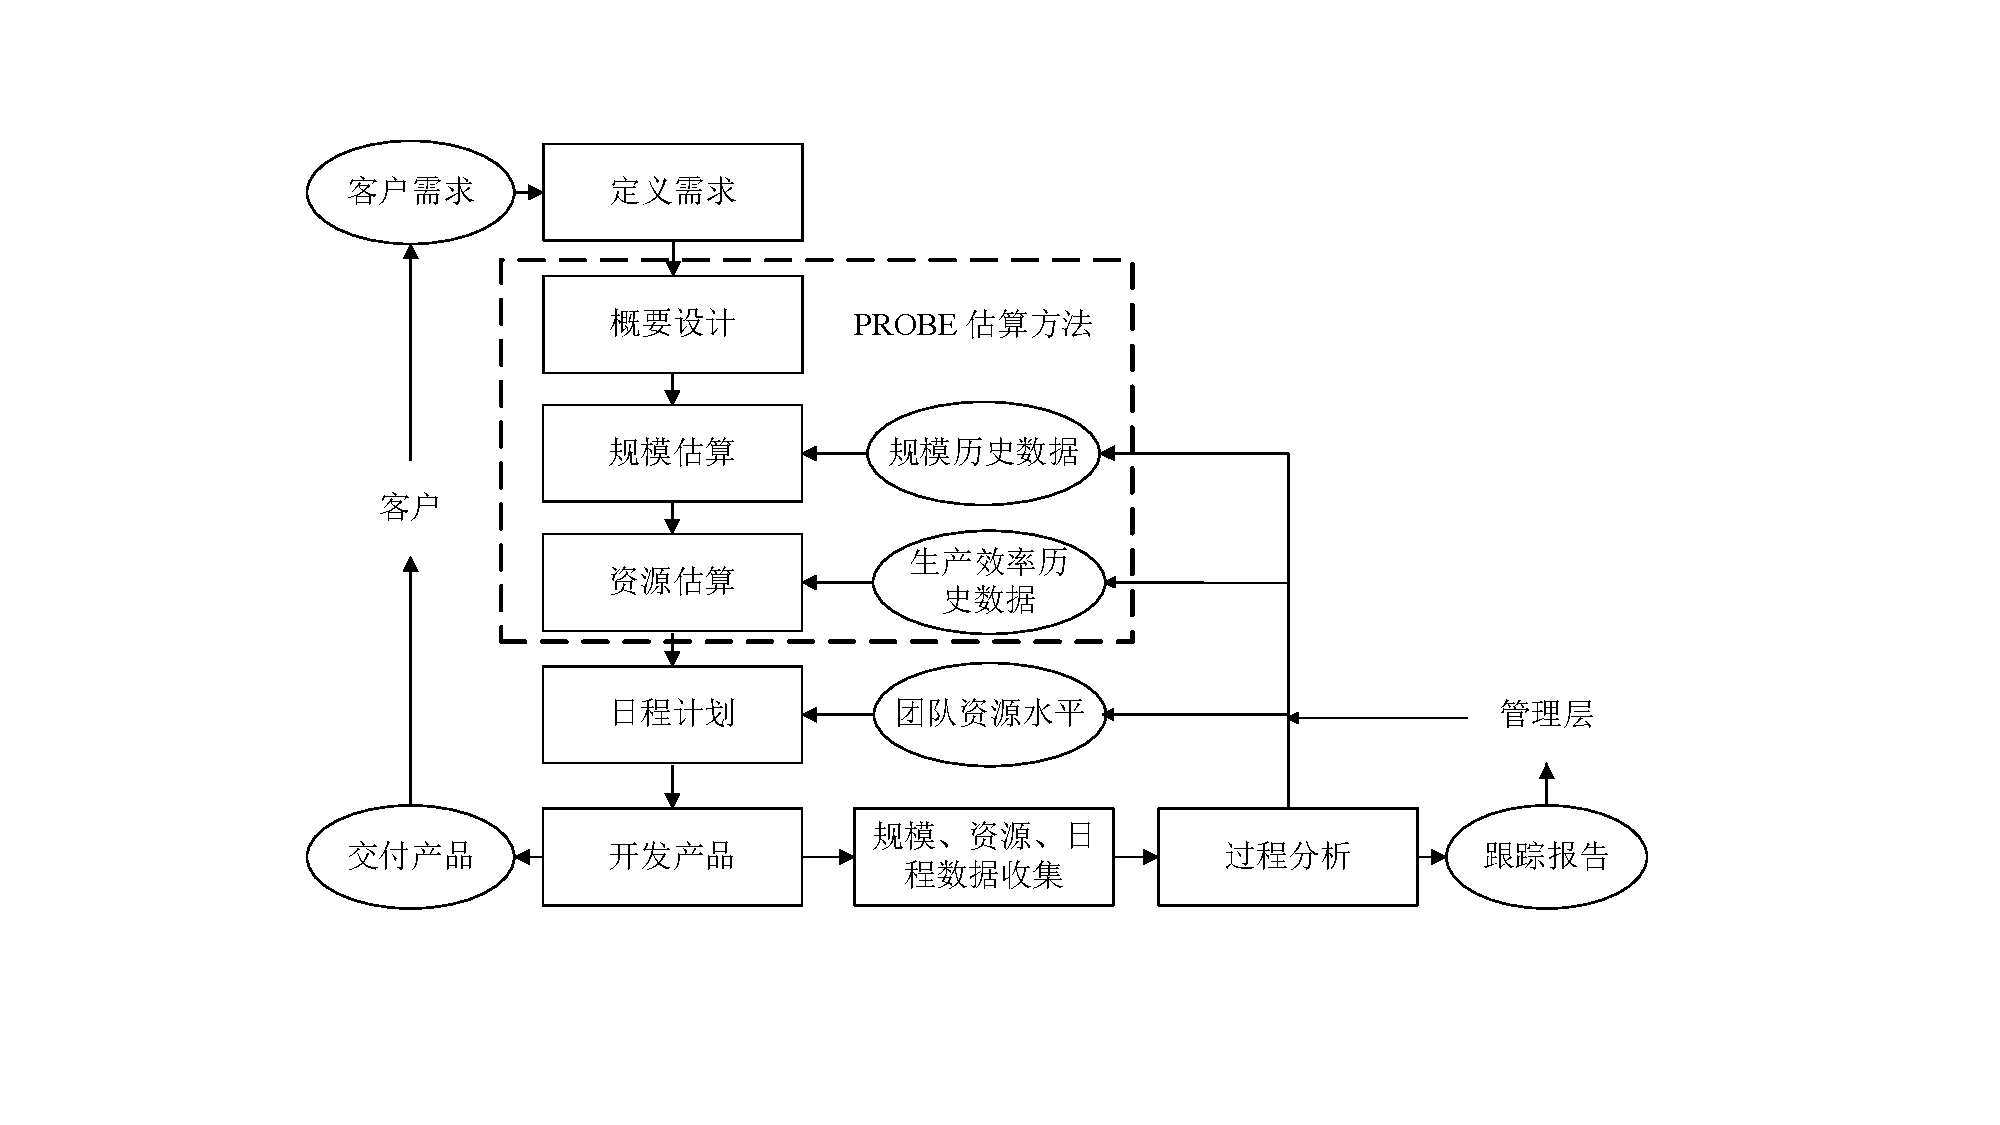
\includegraphics[width=0.5\textwidth]{images/通用计划框架.pdf}
    \vspace{-1em}
\end{figure}
\end{problem}

\begin{problem}
应对风险的典型策略有哪些?请举例说明。
\end{problem}

\begin{problem}
为了确保最终软件产品的质量,在项目计划阶段应该注意哪些问题?
\end{problem}

\subsection{团队项目规划:TSP项目启动}

\subsubsection{TSP的九次会议}
\begin{figure}[H]
    \vspace{-0.5em}
	\centering
	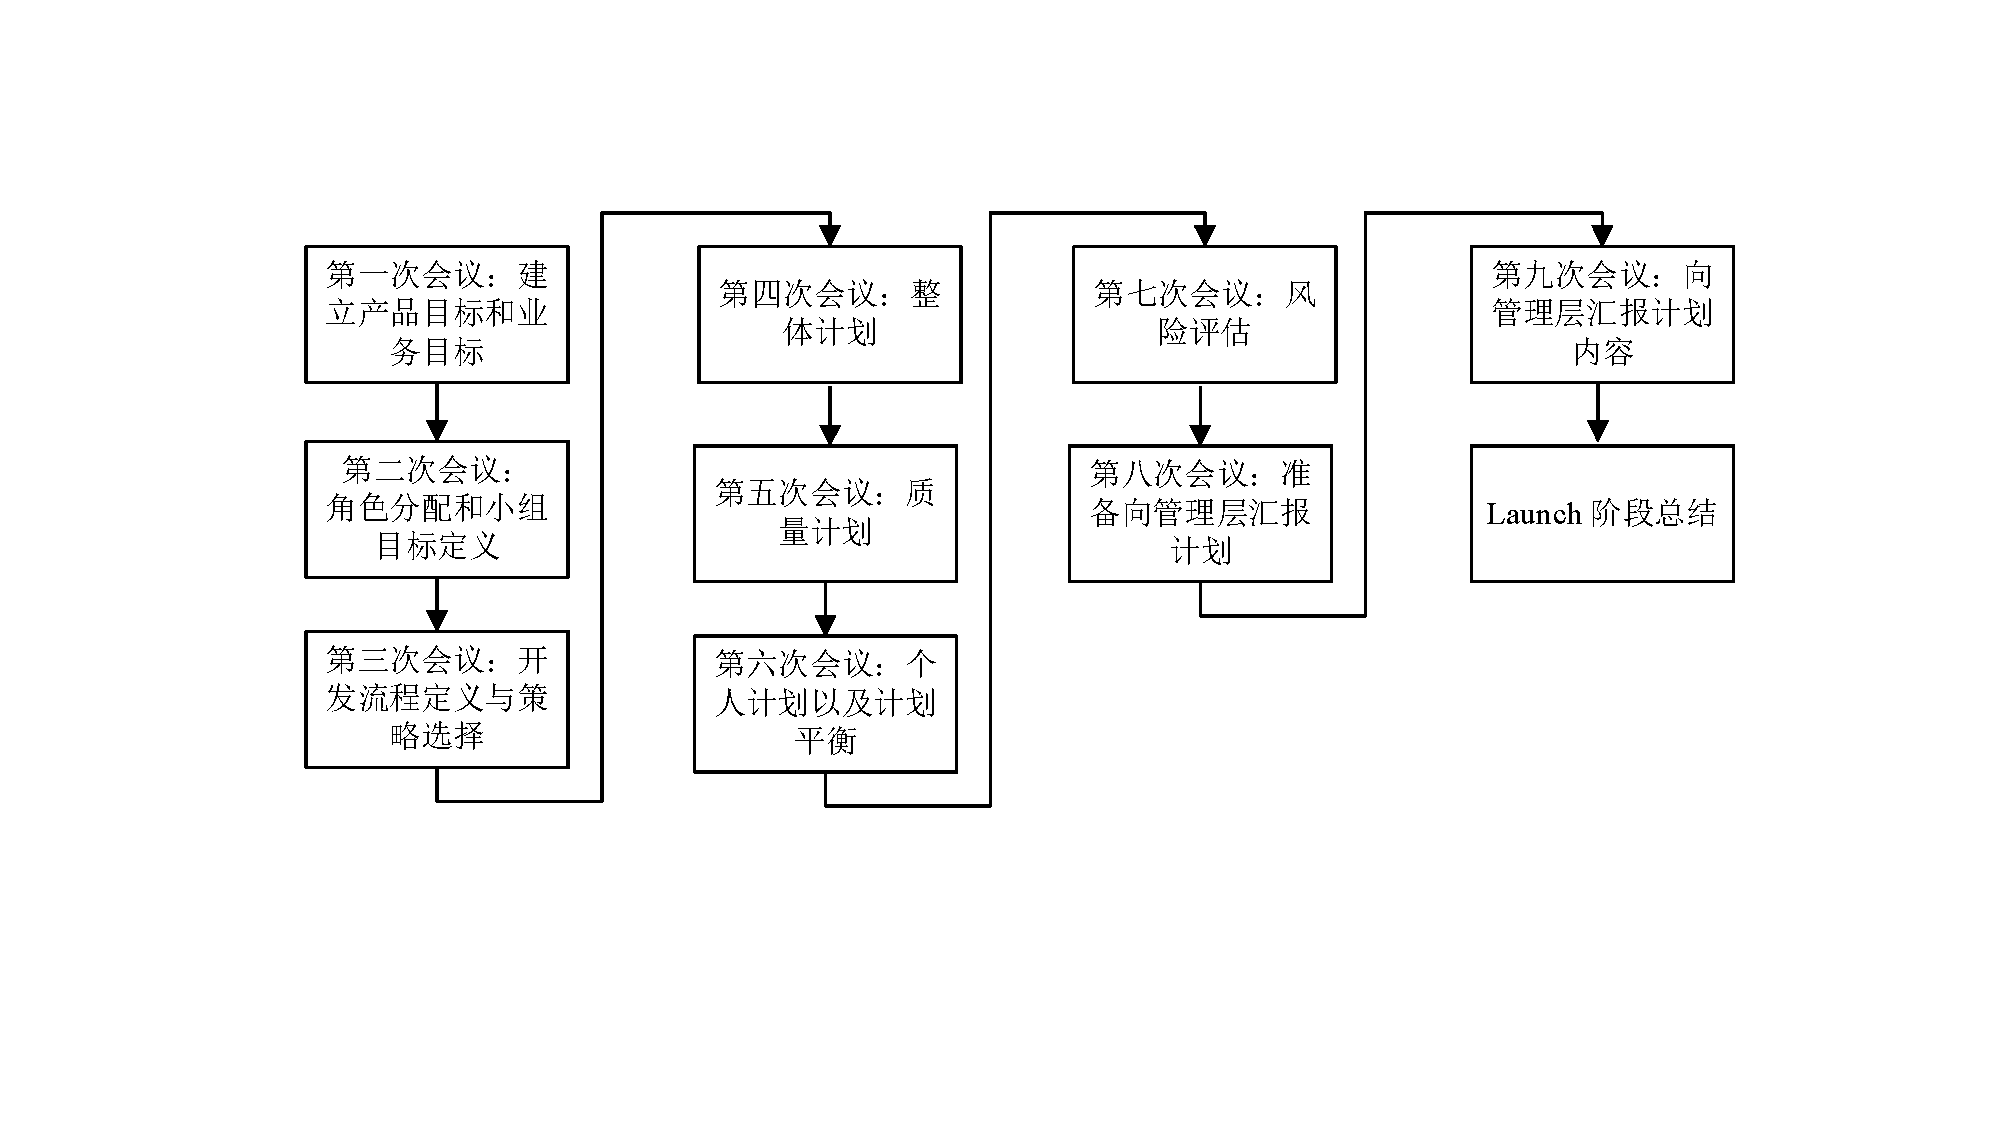
\includegraphics[width=0.85\textwidth]{images/TSP的九次会议.pdf}
    \vspace{-1em}
\end{figure}
几个认识:
\begin{itemize}
    \item 错误的认识:软件开发阶段理解为注入缺陷的阶段,软件测试阶段理解为消除缺陷的阶段
    \item 正确的认识:开发和测试都是既有可能引入缺陷,也有可能消除缺陷的阶段
\end{itemize}

项目完成的实际时间由什么决定?最晚完成的工作的人决定的

经过平衡的计划和没有平衡的计划有什么不一样?更有把握去成功

\subsubsection{考试题目}
\begin{problem}
	在 TSP 的团队组建过程中,确定软件开发策略的是第几次会议?
	\uline{C}    
    \vspace{-0.8em}
    \begin{multicols}{4}
        \begin{enumerate}[label=\Alph*.]
            \item 第一次
            \item 第二次
            \item 第三次
            \item 第四次
        \end{enumerate}
    \end{multicols}
    \vspace{-1em}
\end{problem}

\subsection{团队项目跟踪与分析}
\subsubsection{项目跟踪意义}
在项目进展过程中开展跟踪活动的目的在于了解项目进度,以便在项目实际进展和计划产生严重偏差时,可采取适当的纠正措施
\vspace{-0.8em}
\begin{multicols}{2}
    \begin{itemize}
        \item 项目进度滞后与是否需要参照物,即项目计划
        \item 项目跟踪需要管理偏差而采取的纠偏措施
    \end{itemize}
\end{multicols}
\vspace{-1em}

团队项目的跟踪与管理主要包括进度的跟踪(利用不同跟踪方法,例如挣值管理、里程碑评审)、纠偏活动管理

\subsubsection{项目的挣值管理方法}
\paragraph{什么是EVM}~{} \par
项目的挣值管理方法(EVM, Earned Value Managerment)是用来\textbf{客观度量项目进度}的一种项目管理方法
\vspace{-2.2em}
\begin{multicols}{2}
    \begin{itemize}
        \item 每项任务实现附以一定价值(credit)
        \item 100\%完成该项任务,就获得相应的价值
    \end{itemize}
\end{multicols}
\vspace{-1em}

EVM采用与\textbf{进度计划}、\textbf{成本预算}和\textbf{实际成本}相联系的三个独立的变量,进行项目绩效测量

\paragraph{挣值管理实现}~{} \par
\textbf{简单实现}:仅仅关注进度信息
\begin{itemize}
    \item 实现方式
    \begin{itemize}
        \item 首先需要建立WBS,定义工作范围
        \item 其次为WBS中每一项工作定义一个计划价值(PV, Planned Value)
        \item 最后按照一定的规则将某一数值赋给已经完成的工作或者正在进行的工作,该值成为挣值(EV, Earned Value)
    \end{itemize}
    \item 常用规则
    \begin{itemize}
        \item 0-100原则:只有当某项任务完成时,该任务的PV值将转化成EV值
        \item 50-50原则:只需要开始某项任务,即可以赋原PV值的50\%作为EV值,完成时,再加上另外的50\%
        \item 实际完成的工作所需成本AC不对EV值产生任何影响
    \end{itemize}
\end{itemize}

\textbf{中级实现}
\begin{itemize}
    \item 在简单实现的基础上,加入日程偏差的计算,加入了成本线(AC)
    \item 典型计算方式有
    \vspace{-0.8em}
    \begin{multicols}{2}
        \begin{itemize}
            \item 日程偏差SV = EV $-$ PV
            \item 日程偏差指数SPI = EV/PV;
        \end{itemize}
    \end{multicols}
    \vspace{-1em}
\end{itemize}

\textbf{高级实现}:添加预测线(BAC),当任务足够多的时候,我们就可以让预测线尽可能平直,同时我们延伸挣值(EV),找到与预测线(BAC)的交点,我们就可以明确项目的落后时间

\paragraph{挣值管理图解}~{} \par
\begin{figure}[H]
    \vspace{-0.5em}
	\centering
	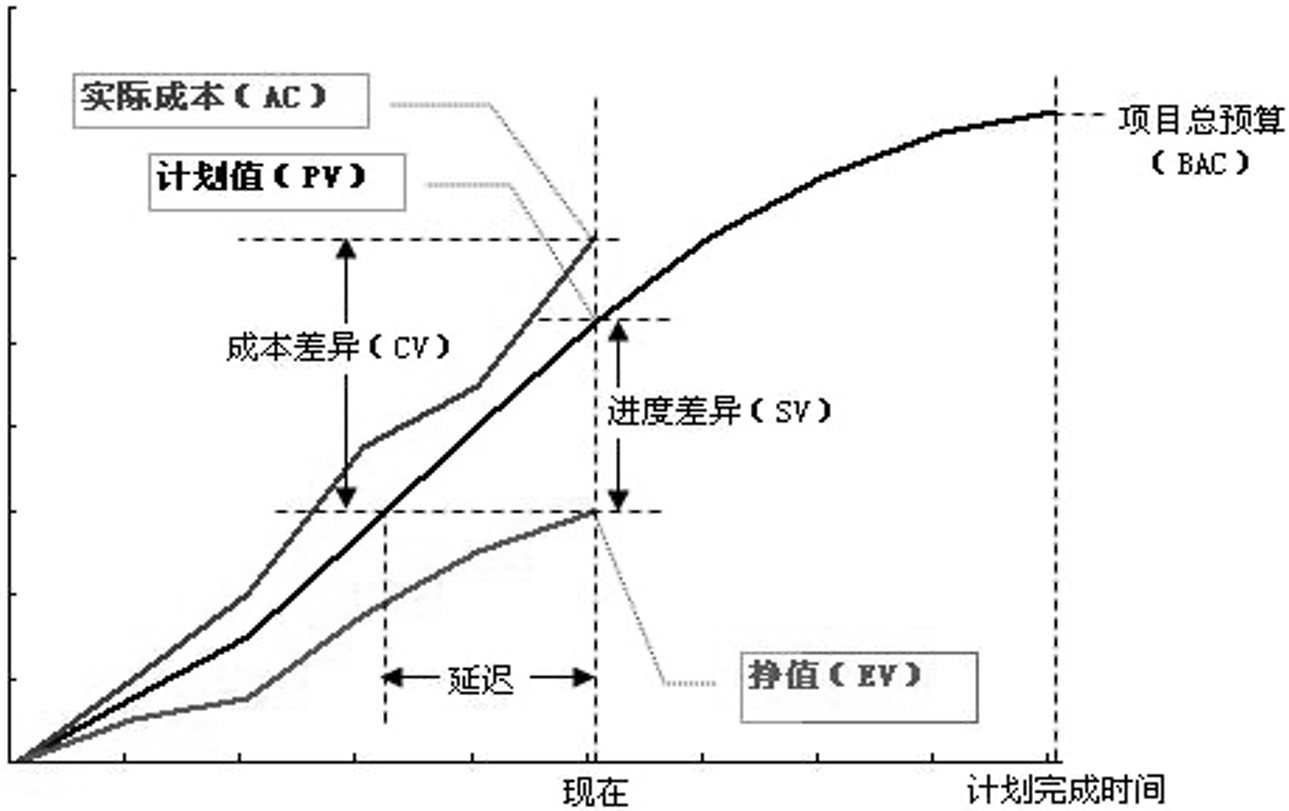
\includegraphics[width=0.6\textwidth]{images/挣值管理图解.png}
    \vspace{-1em}
\end{figure}

\begin{itemize}
    \item 上面的线是为了获取这些挣值付出的实际代价,这个线和挣值之间的差异是成本差异
    \item 中间的线是预算(每天需要完成多少挣值)BAC,理想情况下是一条直线
    \item 下面的线是挣值(实际的进展情况)EV,和owner value有关,对应plan value
    \item 实际获取挣值和预计获取挣值的差异是进度差异
    \item 挣值管理会带来什么好处?可以很好的适应项目的动态变化
\end{itemize}

\paragraph{挣值管理的度量}~{} \par
\begin{itemize}
    \item BAC表示按照PV值的曲线,当项目完成的时候所需预算或者时间
    \item 成本差异CV = EV $-$ AC,表示的是已经完成的工作与所消耗的成本的差异。可以表示为消耗的时间,也可以表示为消耗的资金
    \item 成本差异指数CPI = EV/AC,表示单位成本创造的价值
    \begin{itemize}
        \item CPI < 1说明成本超支;CPI = 1说明成本与预期一致;CPI > 1说明成本低于预期
    \end{itemize}
    \item 日程偏差SV = EV $–$ PV,表示进度偏差
    \begin{itemize}
        \item SV < 0表示进度落后;SV = 0表示进度正常;SV > 0表示进度超前
    \end{itemize}
    \item 日程偏差指数SPI = EV/PV
    \item 预计完成成本EAC = AC + (BAC $-$ EV)/CPI = BAC/CPI,表示的是按照目前的进展已经成本消耗情况,整个项目完成的时候所需消耗的成本
\end{itemize}

\paragraph{挣值管理的应用}~{} \par
发现项目已经滞后
\vspace{-0.8em}
\begin{multicols}{2}
    \begin{itemize}
        \item 削减功能,使得已经完成的任务的EV值增加
        \item 通过加班或加人等手段,提升获取EV值速度
    \end{itemize}
\end{multicols}
\vspace{-1em}

\textbf{例:}EV值显示的项目落后可能是假象,在实际项目过程中,可以采用周报数据的形式来跟踪 EV 值

\begin{wraptable}{r}{0.5\textwidth}
    \centering
    \vspace{-1em}
    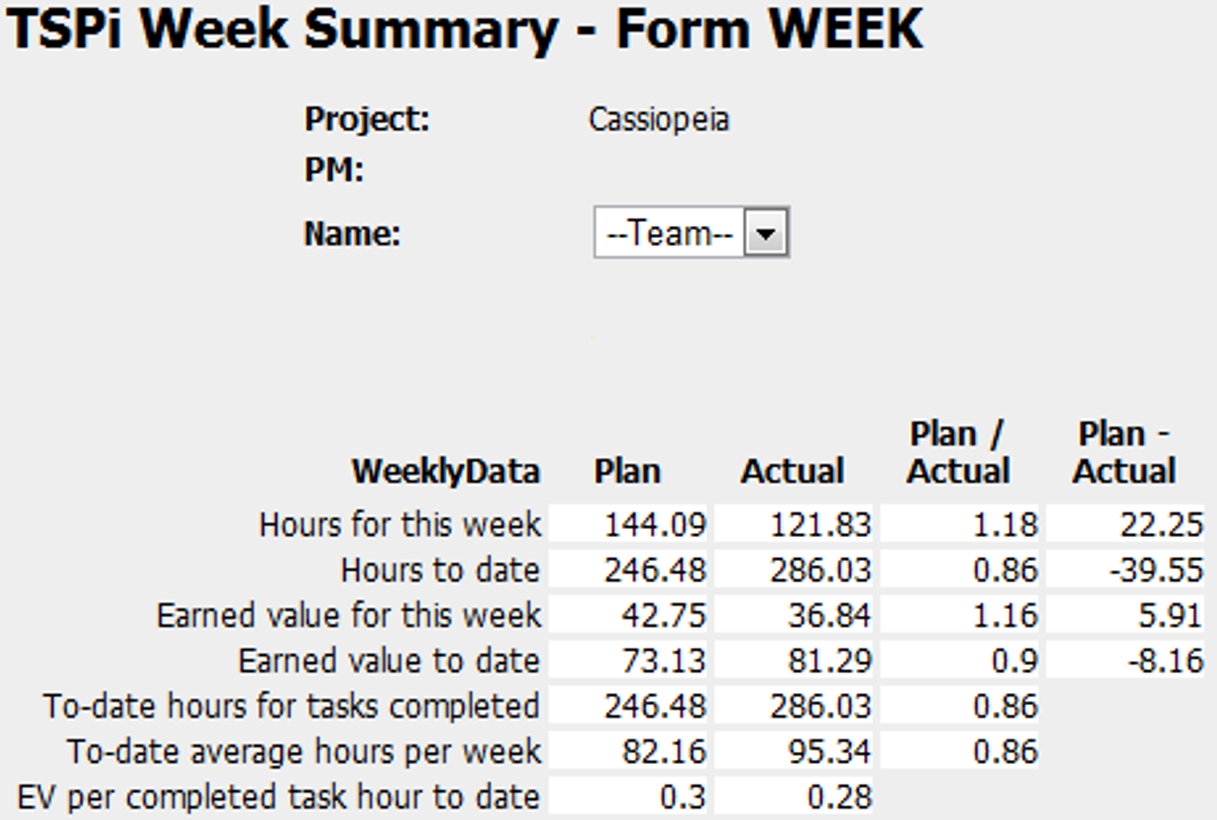
\includegraphics[width=0.5\textwidth]{images/EVM应用示例.png}
    \vspace{-3.5em}
\end{wraptable}
基于图表事实,基本可以得出如下结论:
\begin{itemize}
    \item 项目小组的工作略有提前
    \item 从整体看,项目小组的估算略有偏差,低估了工作难度
    \item 之所以项目目前进度仍然超前,是由于整个团队投人了比预计更多的资源
    \item 按照项目目前的进展情况,整个团队不需要调整,甚至可以相对于以前数周的工作负荷适当减轻负荷
\end{itemize}

\paragraph{挣值管理的局限性}~{} \par
\begin{itemize}
    \item 一般不能应用软件项目的质量管理
    \item 需要定量化的管理机制,这就使得在一些探索型项目以及常用的敏捷开发方法中的应用受到限制
    \item 完全依赖项目的准确估算,然而在项目早期,很难对项目进行非常准确的估算
\end{itemize}

\paragraph{另一种挣值管理变形:燃尽图}~{} \par
\begin{figure}[H]
    \vspace{-0.5em}
	\centering
	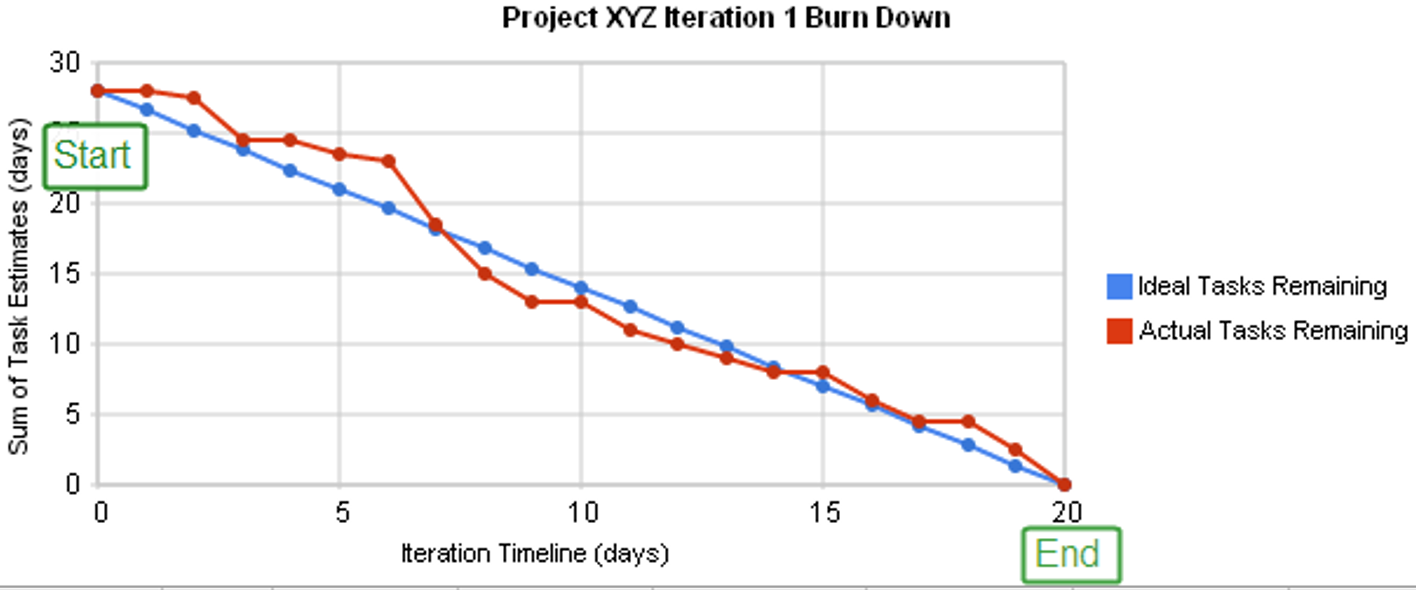
\includegraphics[width=0.63\textwidth]{images/燃尽图}
    \vspace{-1em}
\end{figure}
燃尽图是简单的挣值管理的变形,是剩下的工作占的百分比

\paragraph{考试题目}~{} \par
\begin{problem}
	下列关于挣值管理方法的描述中错误的是?
	\uline{C}    
    \vspace{-0.8em}
    \begin{multicols}{2}
        \begin{enumerate}[label=\Alph*.]
            \item 这是一种可以用来跟踪项目预算消耗的方法
            \item 这种方法高度依赖估算准确性
            \item 这种方法可以支持质量管理
            \item 这种方法可以用来跟踪项目进度
        \end{enumerate}
    \end{multicols}
    \vspace{-1em}
\end{problem}

\subsubsection{里程碑评审}
软件项目的里程碑往往是指某个时间点,用以标记某些工作的完成或者阶段的结束。典型的里程碑事件:
\vspace{-0.8em}
\begin{multicols}{4}
    \begin{itemize}
        \item 完成某项工作
        \item 获干系人签字认可
        \item 完成某产物的评审
        \item 修改或交付某产物
    \end{itemize}
\end{multicols}
\vspace{-1em}

里程碑评审的审查内容包括:
\vspace{-0.8em}
\begin{multicols}{2}
    \begin{itemize}
        \item 项目相关的承诺,如日期、规格、质量等等
        \item 项目各项计划的执行状况
        \item 项目当前的状态讨论
        \item 项目面临的风险讨论等
    \end{itemize}
\end{multicols}
\vspace{-1em}

里程碑评审也可用于质量管理

\subsubsection{其他类型跟踪方法}
\vspace{-0.8em}
\begin{multicols}{3}
    \begin{itemize}
        \item 日程计划跟踪
        \item 承诺计划跟踪
        \item 风险计划跟踪
        \item 数据收集计划跟踪
        \item 沟通计划跟踪
    \end{itemize}
\end{multicols}
\vspace{-1em}

\subsubsection{纠偏活动的管理}
典型的纠偏活动包括:偏差原因分析、纠偏措施定义、纠偏措施管理
\begin{itemize}
    \item 偏差原因分析:收集偏差相关的各种信息,基于收集到的信息,开展充分的分析工作,找出偏差的根本原因
    \item 纠偏措施定义:确认偏差的根本原因,就可以有针对性地定义纠偏的措施
    \item 纠偏措施管理:管理纠偏措施直到结项
\end{itemize}

\subsubsection{项目审查}
审查的内容包括:
\vspace{-0.8em}
\begin{multicols}{3}
    \begin{enumerate}[label=\arabic*.]
        \item 项目相关的承诺,如日期、规格、质量等等
        \item 项目各项计划的执行状况
        \item 项目当前的状态讨论
        \item 项目面临的风险讨论
        \item 其他计划跟踪
        \item 日程计划跟踪
        \item 承诺计划跟踪
        \item 风险计划跟踪
        \item 数据收集计划跟踪
        \item 沟通计划跟踪
    \end{enumerate}
\end{multicols}
\vspace{-1em}

\subsection{项目总结}
\subsubsection{项目总结的定义}
\begin{itemize}
    \item 项目总结需要系统化有条理的进行,才能不遗漏重要的内容
    \item 因此往往需要事先定义总结过程,然后就按部就班地开展总结工作
\end{itemize}

\subsubsection{一般项目总结流程}
基于PMBOK的总结方式,包含范围管理、时间管理、成本管理、质量管理、人力资源管理、沟通管理、风险管理、采购管理和整合管理9大知识领域
\begin{enumerate}[label=\arabic*.]
    \item 项目范围包括产品范围和项目范围。对项目范围管理的总结应当主要关注项目的需求开发过程与变更管理中的得失,对需求管理实际执行情况的差距进行原因分析,找到改进的机会
    \item 时间管理所关注的就是项目的日程计划以及对日程计划的跟踪和管理状况。因此主要考察计划的准确程度以及各个里程碑的偏差情况
    \item 成本管理包括对成本进行估算、预算和控制的各个过程,从而确保项目在批准的预算内完工
    \item 质量管理包括执行组织确定质量政策、目标与职责的各过程和活动,从而使项目满足其预定的需求
    \item 人力资源管理包括组织、管理与领导项目团队的各个过程
    \item 沟通管理包括为确保项目信息及时且恰当地生成、收集、发布、存储、调用最终处置所需的各个过程
    \item 风险管理包括风险管理规划、风险识别、风险分析、风险应对规划和风险监控等各个过程
    \item 采购管理包括从项目组织外部采购或获得所需产品、服务或成果的各个过程
    \item 整合管理包括为识别、定义、组合、统一与协调项目管理过程组的各过程及项目管理活动而进行的各种过程和活动
\end{enumerate}

\subsubsection{TSP项目总结方式}
\begin{enumerate}[label=\arabic*.]
    \item 准备阶段
    \item 过程数据评审阶段:该阶段往往由过程经理或者质量经理带领整个团队分析过程数据,识别过程改进机会
    \begin{itemize}
        \item 可以结合典型TSP团队角色,逐个讨论改进领域。如团队领导力、计划准确性、过程优劣、质量管理能力、开发环境以及配置管理等。
        \item 此外,也可以就TSP教练的作用进行评价。
        \item 过程数据评审阶段还要求开发团队的所有成员都整理过程改进提案(PIP):PIP是TSP过程中供开发人员在日程工作中记录改进想法的工具。其基本思想是积累小的改进,慢慢形成大的改进。在软件开发过程中,重大的改进机会不多,因此,往往需要从小做起,慢慢积累之后,就会形成对原有过程的显著改进。小的改进机会虽然多,但是容易被遗忘,PIP的作用就在于提供了一个标准表格工具,允许软件工程师时时记录改进方案。在项目总结阶段,将开发过程中记录的所有PIP整理出来,形成整个开发周期的过程改进提案,供讨论,以确定下个开发周期要实施的过程改进。
    \end{itemize}
    \item 人员角色评价阶段(角色包括项目组长、计划经理、开发经理、质量经理、过程经理和支持经理)
    \item 总结报告撰写阶段
\end{enumerate}

\subsubsection{通用项目总结流程}
\vspace{-0.8em}
\begin{multicols}{3}
    \begin{enumerate}[label=\arabic*.]
        \item 准备阶段
        \item 总结阶段
        \item 报告阶段
    \end{enumerate}
\end{multicols}
\vspace{-1em}

\subsubsection{项目总结的意义}
提供一个系统化的方式来总结经验教训、防止犯同样的错误、评估项目团队绩效、积累过程数据等,给项目团队成员持续学习和改进的机会

\subsection{项目管理支持活动}
项目管理支持活动包含:配置管理、度量和分析、决策分析和根因分析

\subsubsection{配置管理}
\paragraph{配置管理的目的}~{} \par
建立与维护工作产品的完整性

\paragraph{配置管理的概念}~{} \par
配置项:
\begin{itemize}
    \item 在配置管理当中作为单独实体进行管理和控制的工作产品集合
    \item 典型的可能作为配置项纳入配置管理的工作产品包含过程说明文档、项目开发计划文档、需求规格说明书、设计规格说明书、设计图表、产品规格说明书、程序代码、开发环境,如特定版本的编译器等、产品数据文件、产品技术文件、用户支持文档
\end{itemize}

基线:基线是一个或多个配置项及相关的标识符的代表,是一组经正式审查同意的规格或工作产品集合,是未来开发工作或交付的基础,而且只能经由严格的变更控制程序才能改变
\begin{itemize}
    \item 发布一个基线包括该基线所有的配置项以及这些配置项的最新变更,因此,可以将基线作为接下来工作的基础
    \item 典型的发布基线时间点为需求分析之后、设计完成之后、单元测试之后以及最终产品发布
    \item 是配置项持续演进的稳定基础
\end{itemize}

\paragraph{配置管理的流程}~{} \par
配置管理是用管理的手段监督和指导如下工作的流程[CMMI 2006]
\vspace{-0.8em}
\begin{multicols}{2}
    \begin{enumerate}[label=\arabic*.]
        \item 识别和记录配置项的物理特性和功能特性
        \item  控制上述特性的变更
        \item 记录和报告变更过程和相应的配置项状态
        \item 验证配置项是否与需求一致
    \end{enumerate}
\end{multicols}
\vspace{-1em}

\begin{wraptable}{r}{0.65\textwidth}
    \centering
    \vspace{-1.5em}
    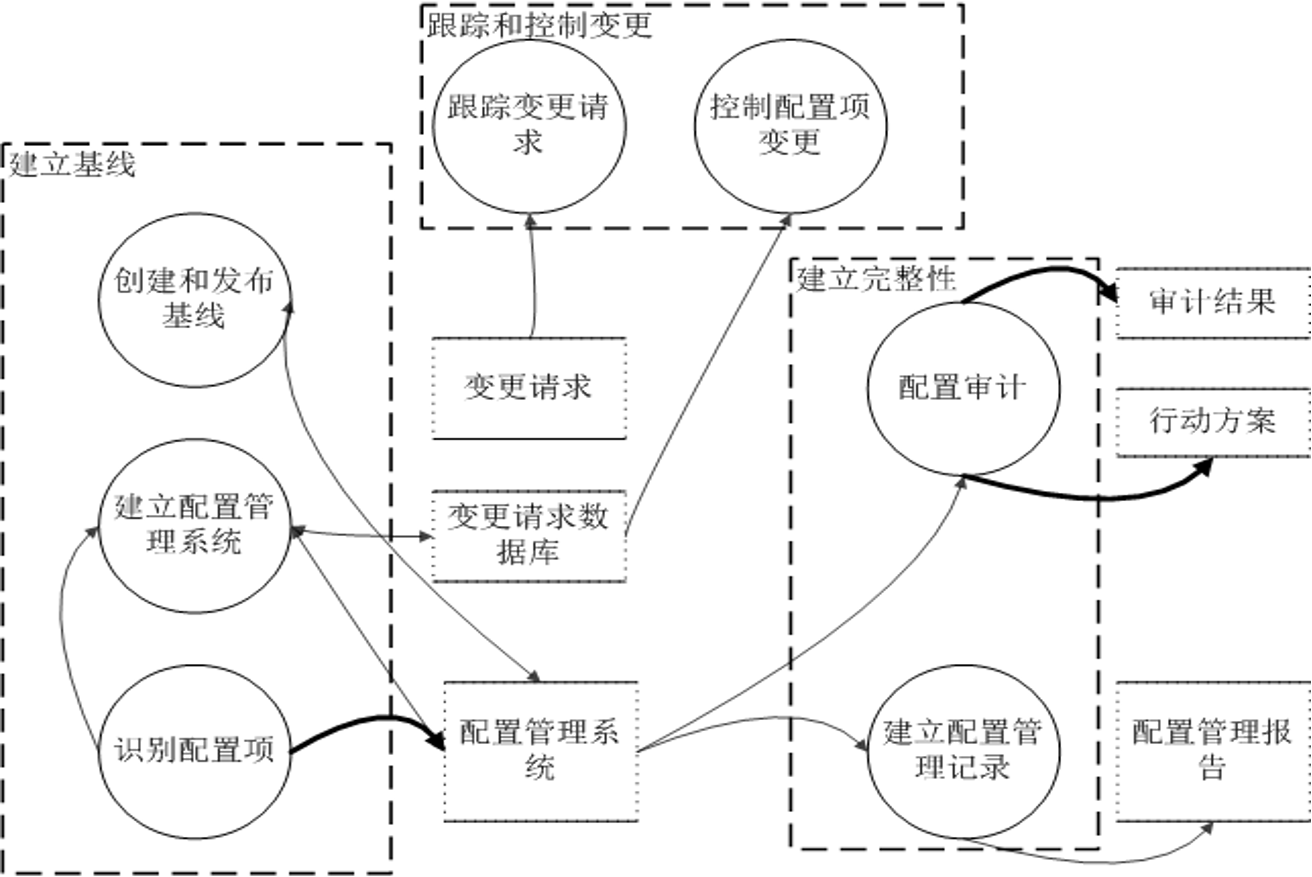
\includegraphics[width=0.55\textwidth]{images/配置管理活动.png}
    \vspace{-5.5em}
\end{wraptable}
\paragraph{配置管理活动}~{} \par
\begin{enumerate}[label=\arabic*.]
    \item 识别配置项
    \item 建立配置管理系统
    \item 创建和发布基线
    \item 跟踪变更请求
    \item 控制配置项变更
    \item 建立配置管理记录
    \item 配置审计
\end{enumerate}

\paragraph{考试题目}~{} \par
\begin{problem}
请解释配置管理中配置项和产品基线的概念,并设计一个流程对单元测试后已经纳入配置库的代码,修改集成测试中的若干问题后,该如何控制变更。

配置项和产品基线的概念如上

如何控制变更:
\begin{itemize}
    \item 跟踪变更请求
    \begin{itemize}
        \item 启动变更请求处理程序,将变更情况保存在变更请求数据库中
        \item 分析变更建议和所需进行的修改将对工作产品、进度、日程等造成的影响
        \item 如果变更请求影响到其他基线,则与相关的干系人一起审查这些变更请求,并取得他们的同意
        \item 跟踪变更申请直到结项
    \end{itemize}
    \item 控制配置项变更
    \vspace{-0.8em}
    \begin{multicols}{2}
        \begin{itemize}
            \item 确认这些修订已得授权
            \item 更新配置项
            \item 将旧基线归档保存,并获取新基线
            \item 执行审查,确保该变更没有对基线造成意料外的影响
            \item 上当记录配置项的变更内容和变更理由
        \end{itemize}
    \end{multicols}
    \vspace{-1em}
\end{itemize}
\end{problem}

\subsubsection{度量和分析}
\paragraph{度量和分析简介}~{} \par
意义:在软件项目管理决策的过程中,基于客观的数据很重要,这种客观决策可以显著消除错误决策的风险。而这些客观数据的获得,必须依照一定的流程以正确的方式获得和使用。度量和分析活动就定义了上述客观数据的获取与使用方式。

目的:建立与维持度量能力,以支持管理的信息需要。

\begin{wraptable}{r}{0.6\textwidth}
    \centering
    \vspace{-2em}
    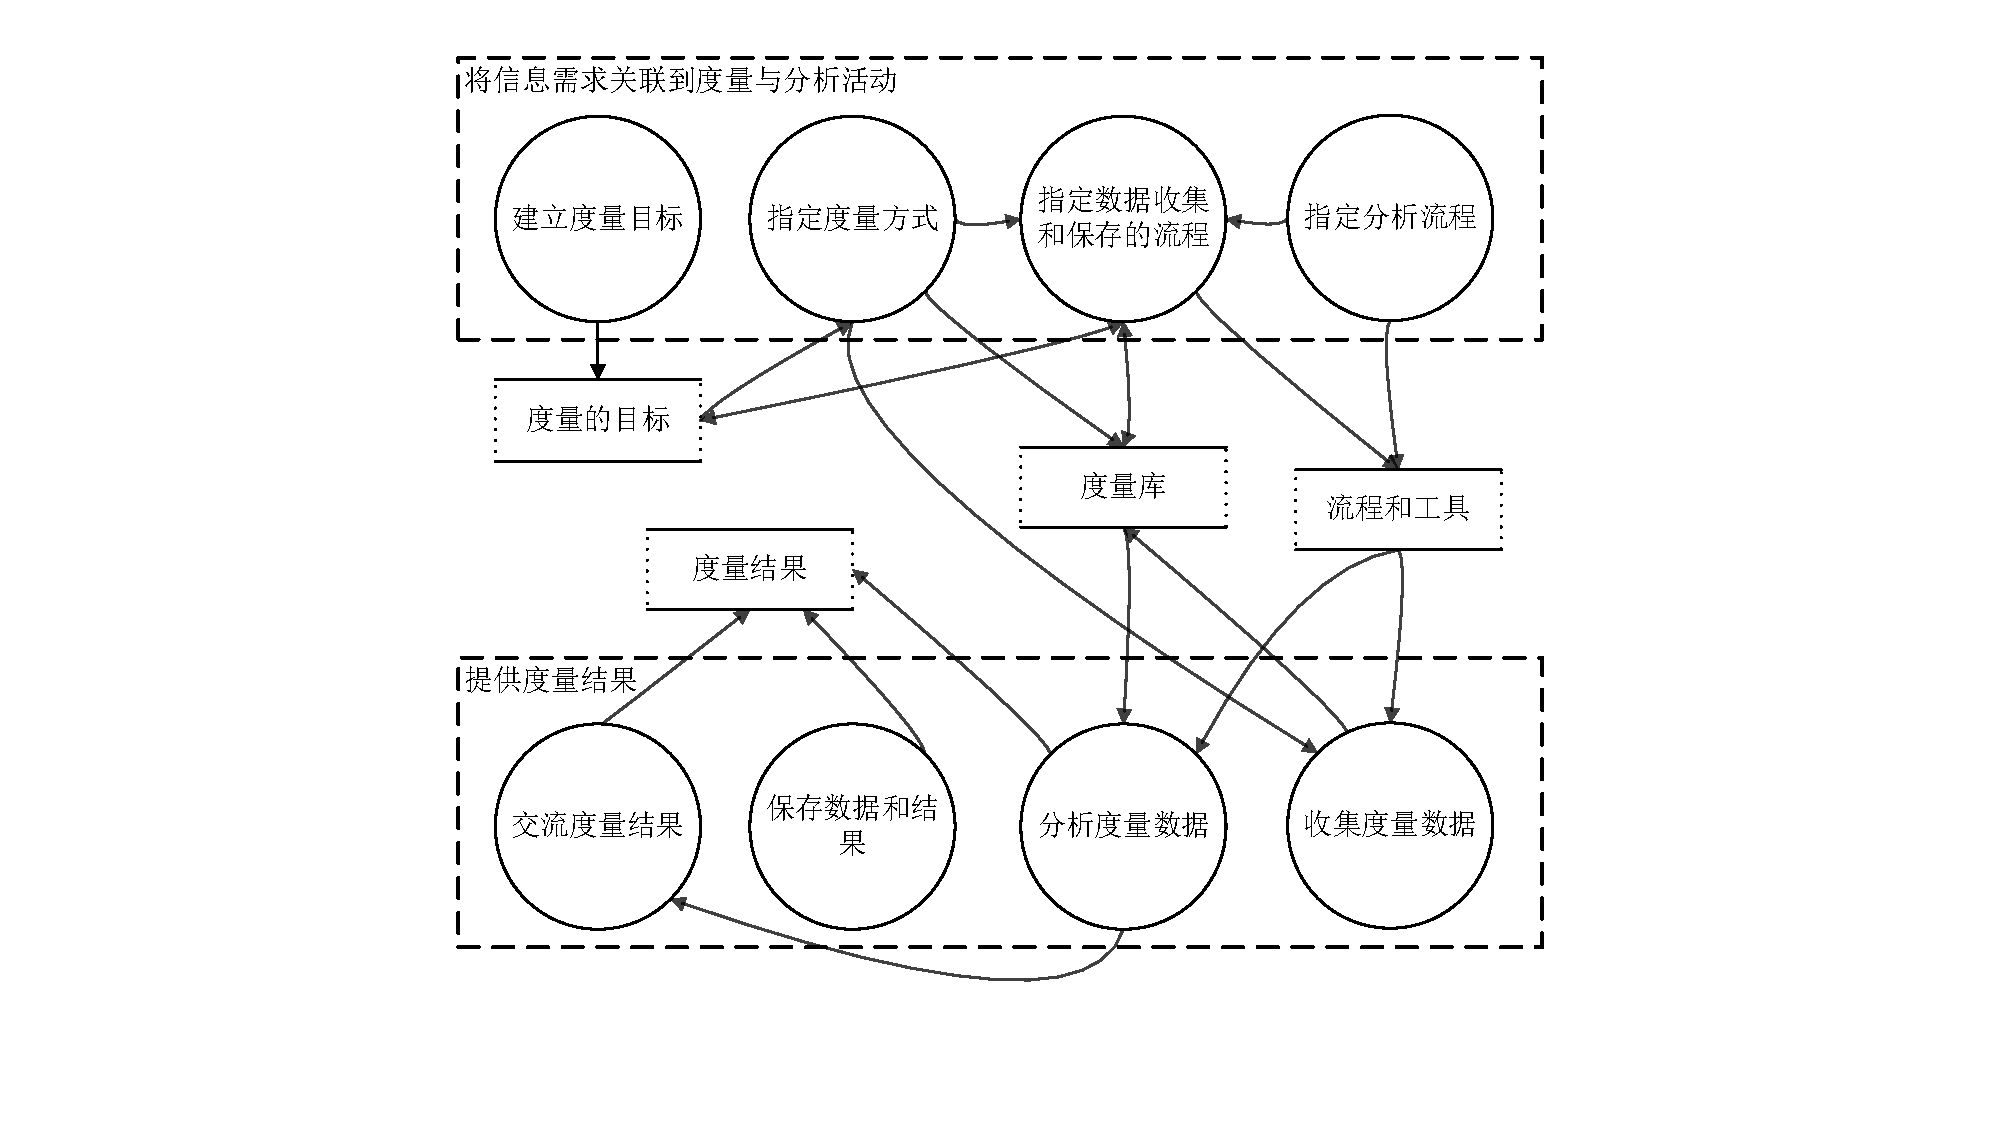
\includegraphics[width=0.6\textwidth]{images/度量与分析活动.pdf}
    \vspace{-7em}
\end{wraptable}
\paragraph{度量和分析活动}~{} \par
\begin{enumerate}[label=\arabic*.]
    \item 建立度量目标
    \item 指定度量方式
    \item 指定数据收集和保存的流程
    \item 指定分析流程
    \item 收集度量数据
    \item 分析度量数据
    \item 保存数据和结果
    \item 交流度量结果
\end{enumerate}

\paragraph{GQM方法的原理和应用}~{} \par
GQM(Goal Question Metric)是一种应用非常广泛的建立软件度量体系的方法,从管理的目标出发,将目标归纳、分解为度量的指标,并把这些指标提炼成可以测量的值,是一种科学的、系统的思考问题的方式
\begin{itemize}
    \item 概念层(目标):目标是为某个特定的对象而定义的。这里的对象是指软件产品、软件过程以及相关的资源等。定义的目标基于不同原因和不同质量模型,也要参考不同的角色视图与特定的环境
    \item 操作层(问题):基于一定的刻画上述目标是否达成或者目标达成的进展情况的模型,使用一系列的问题来定义所研究的对象, 然后得出评价或评估特定目标达成进展情况。所选择的问题应当尽量体现质量相关的话题
    \item 量化层(度量):试图以量化的方式回答上述操作层识别出来的问题
\end{itemize}

\textbf{例:}GQM示例:PM
\vspace{-0.8em}
\begin{multicols}{2}
    \begin{itemize}
        \item G: 确保稳定性、可预测性的开发过程来满足计划的里程碑。
        \item Q: 我的项目是否按照计划的轨迹前进,计划的里程碑都能实现吗?
        \item M: 软件项目开发工作的挥发性(分支、流、变更管理(UCM)活动)。
    \end{itemize}
\end{multicols}
\vspace{-1em}

\textbf{例:}GQM示例:DM
\vspace{-0.8em}
\begin{multicols}{2}
    \begin{itemize}
        \item G: 最大化所有团队贡献者的生产力。
        \item Q: 开发人员能够完成分配给他们的任务吗,或者他们遇到障碍了吗?
        \item M: 由个体或者工作组产生的项目工件的数量
    \end{itemize}
\end{multicols}
\vspace{-1em}

\paragraph{考试题目}~{} \par
\begin{problem}
请结合GQM思想解释PSP过程的基本度量元有哪几个?
\end{problem}

\begin{problem}
描述一下度量和分析活动在一个软件项⽬当中的作用,以及应该如何正确开展?

可以描述度量和分析活动,也可以描述GQM
\end{problem}

\subsubsection{决策分析}
决策分析的意义:错误的决策往往会给项目带来灾难性后果。为了降低这种错误决策的风险,往往需要尽可能基于客观事实和正确的流程来开展决策与分析活动

\begin{wraptable}{r}{0.55\textwidth}
    \centering
    \vspace{-1.5em}
    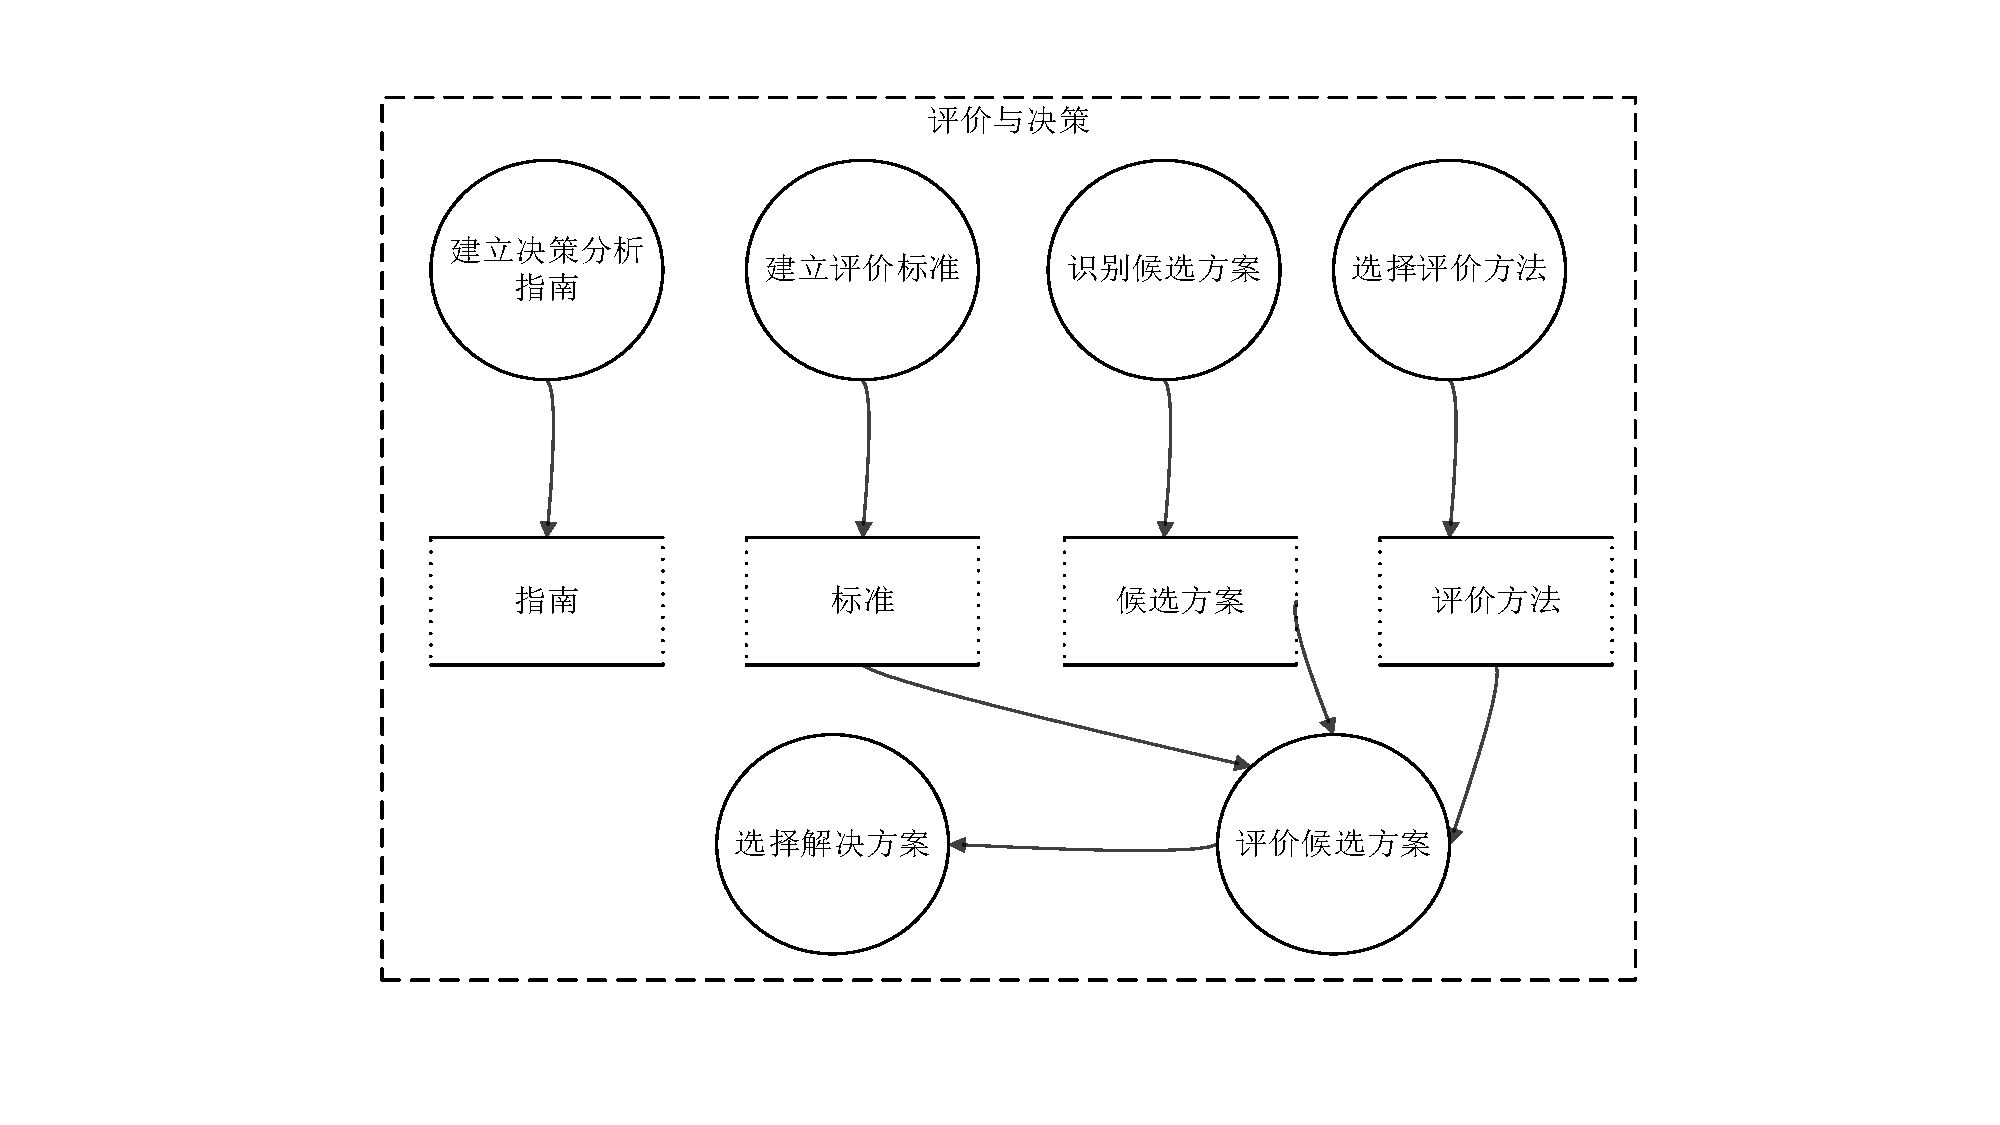
\includegraphics[width=0.55\textwidth]{images/决策分析活动.pdf}
    \vspace{-6.5em}
\end{wraptable}
决策分析往往包含以下活动:
\begin{enumerate}[label=\arabic*.]
    \item 建立决策分析指南
    \item 建立评价标准
    \item 识别候选方案
    \item 选择评价方法
    \item 评价候选方案
    \item 选择解决方案
\end{enumerate}

\subsubsection{根因分析}
避免类似错误反复发生,一个正式根因分析过程往往包含下列的活动:
\vspace{-0.8em}
\begin{multicols}{4}
    \begin{itemize}
        \item 识别和选定问题
        \item 根因分析
        \item 建立改进行动方案
        \item 实施改进,评估效果
    \end{itemize}
\end{multicols}
\vspace{-1em}

\begin{figure}[H]
    \vspace{-0.5em}
	\centering
	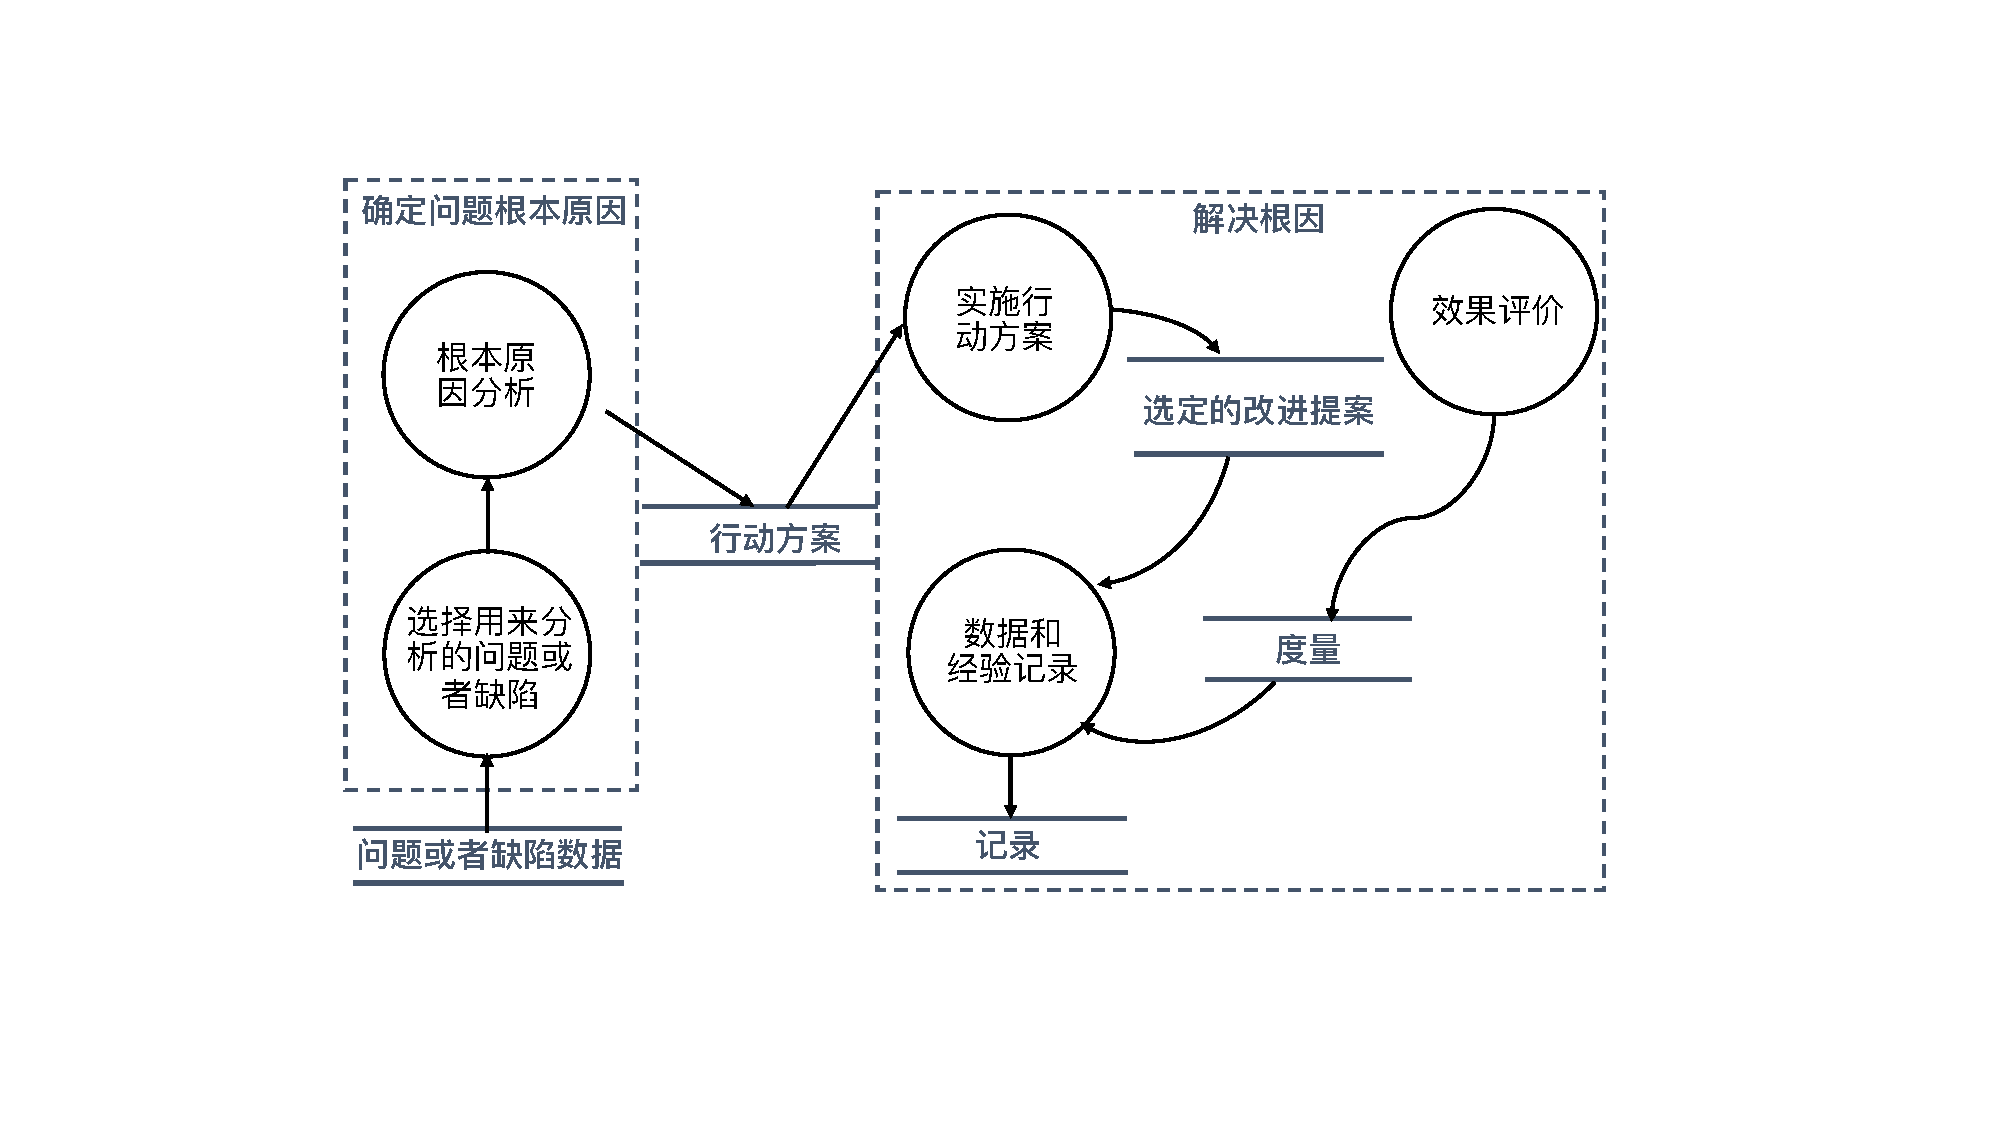
\includegraphics[width=0.63\textwidth]{images/根因分析活动.pdf}
    \vspace{-1em}
\end{figure}
\vspace{-1em}

根因分析典型示例
\begin{figure}[H]
    \vspace{-0.5em}
	\centering
	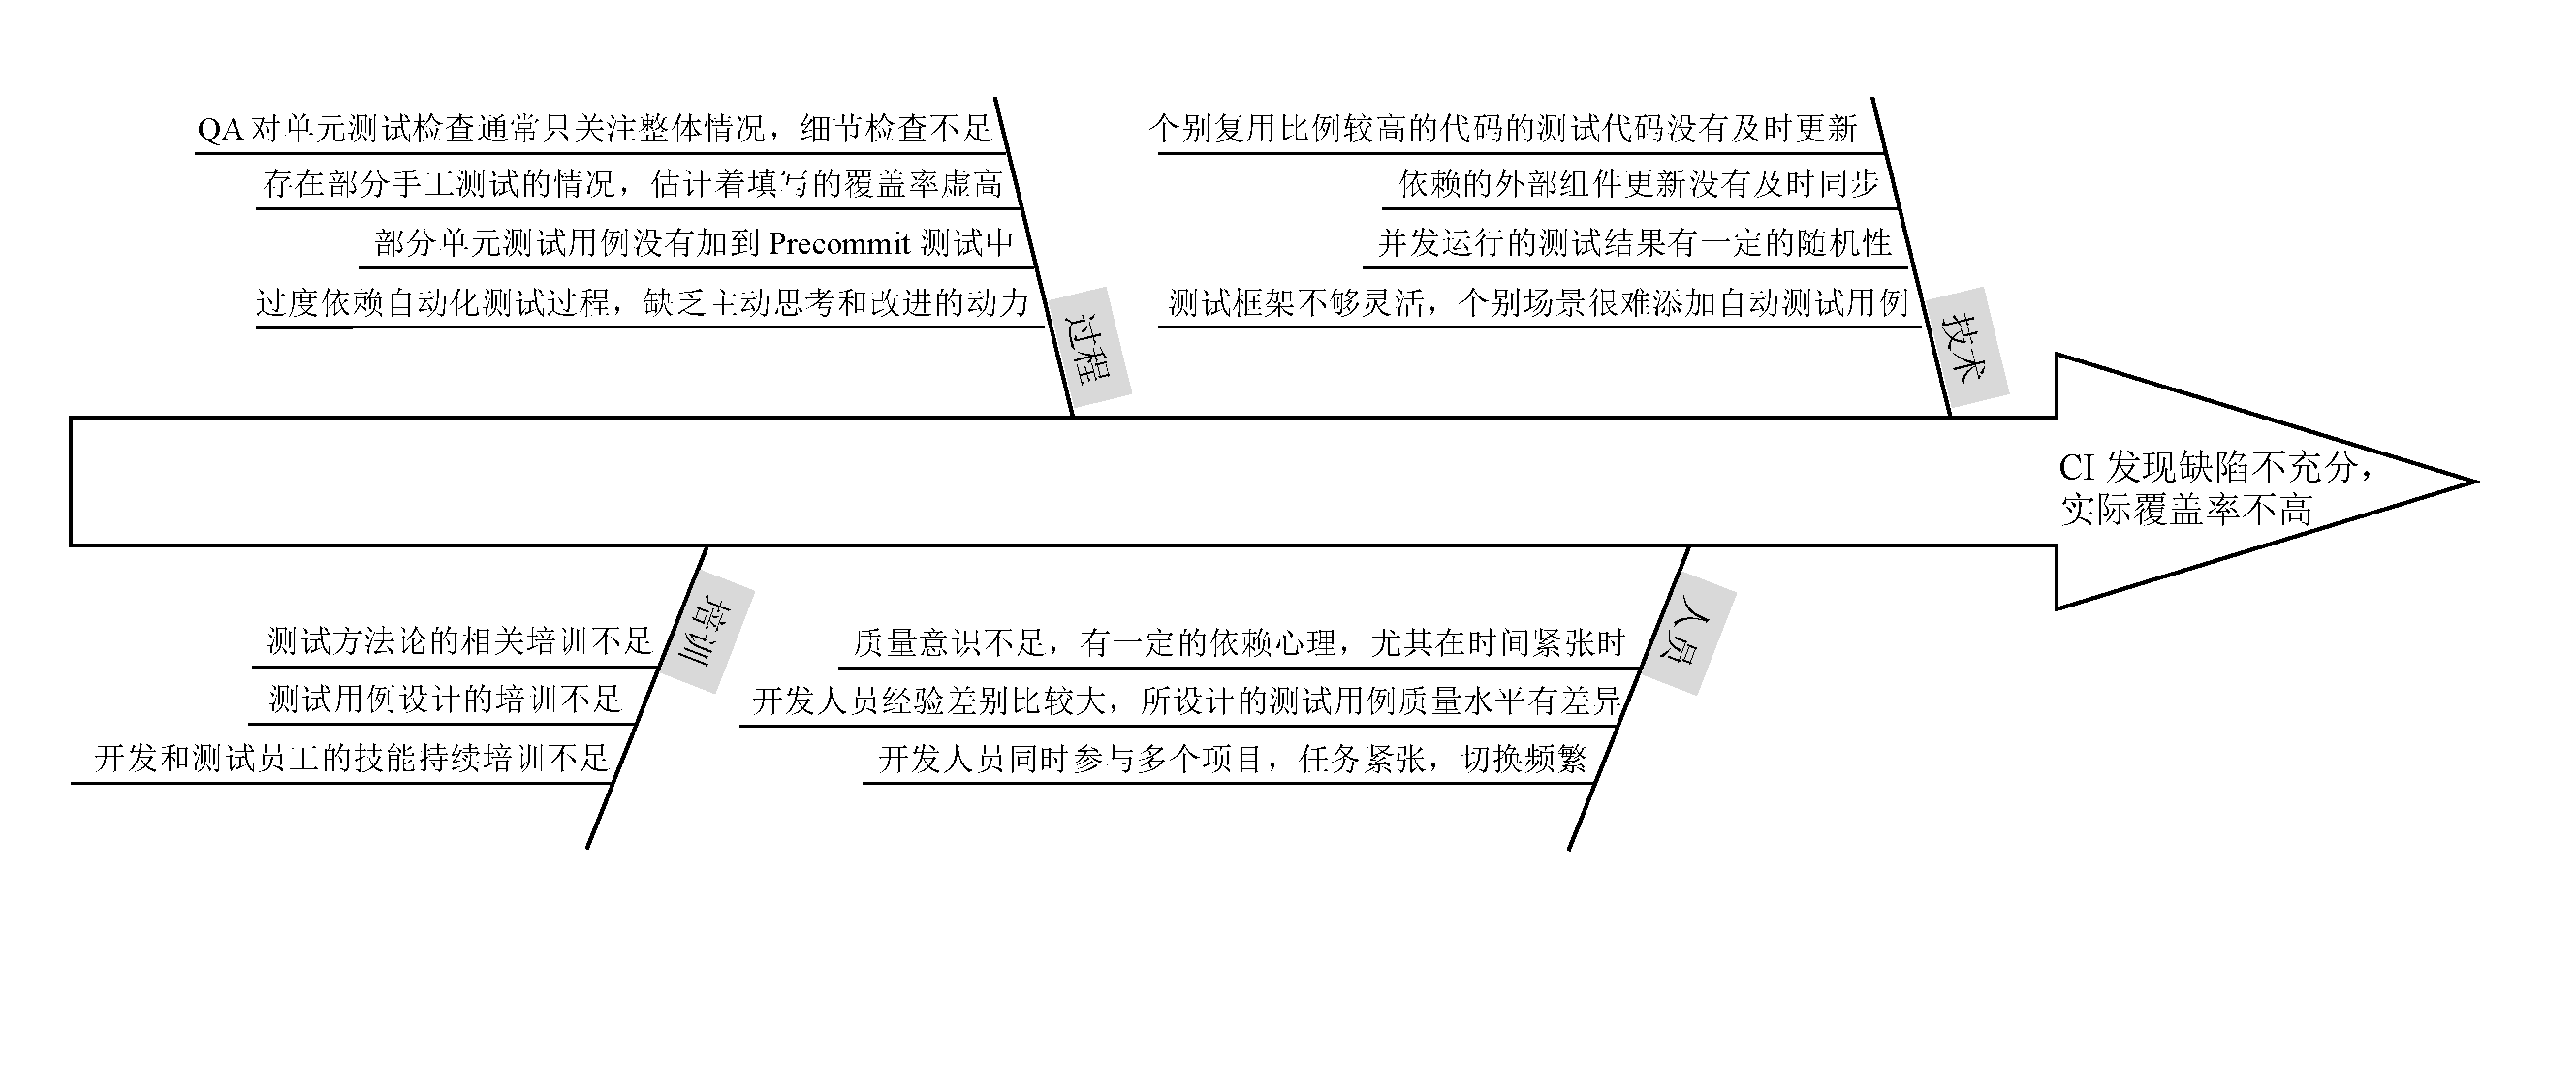
\includegraphics[width=0.9\textwidth]{images/根因分析典型示例.pdf}
    \vspace{-1em}
\end{figure}
\vspace{-1em}

\subsection{团队动力学}
软件开发的特点:
\begin{itemize}
    \item 软件开发是一项\textbf{既复杂又富有创造性}的知识工作
    \item 软件开发:智力劳动,需要处理和讨论极其抽象的概念,并把不同的部分(不可见)整合成一个可以工作的系统
    \begin{itemize}
        \item 要求从事软件开发的工程师
        \begin{itemize}
            \item \textbf{必须全身心地参与工作}:知识工作必须是全身心投入的,任务切换一般需要30分钟才能全身心的投入
            \item \textbf{主观意愿上努力追求卓越}
        \end{itemize}
        \item 要求管理者激励并维持激励:激励手段、维持激励手段
    \end{itemize}
\end{itemize}

管理知识工作的关键规则是:\textbf{管理者无法管理工作者,知识工作者必须实现并学会自我管理}
\begin{itemize}
    \item 要自我管理,知识工作者必须(自我管理的前提条件)
    \vspace{-0.8em}
    \begin{multicols}{3}
        \begin{itemize}
        \item 有积极性
        \item 能做出准确的估算和计划
        \item 懂得协商承诺
        \item 有效跟踪他们的计划
        \item 持续地按计划交付高质量产品
        \end{itemize}
    \end{multicols}
    \vspace{-1em}
    \item 知识工作者实现自我管理:\textbf{胶冻状团队}
\end{itemize}

知识工作者的管理需要的是领导者,而不是经理,领导者需要诚实、有能力、有远见、鼓舞人心

\subsubsection{自主团队}

\paragraph{团队定义}~{} \par
一个团队必须包括至少\textbf{两个成员},他们为了\textbf{共同的目标和愿景}而努力工作,他们每个人都有\textbf{明确的角色}和\textbf{相应的职责定义},任务的完成需要团队成员\textbf{互相依赖和支持}

\paragraph{自主团队的含义}~{} \par
软件工程师所从事的工作一般称之为复杂的知识工作。在这种性质的工作中,实现软件工程师的自我管理往往可以获得最好的工作效率和质量水平。如果整个团队的所有成员都实现了自我管理,也就形成了所谓的自主团队。

\paragraph{自主团队的特点}~{} \par
\vspace{-0.8em}
\begin{multicols}{3}
    \begin{enumerate}[label=\arabic*.]
        \item 自行定义项目的目标
        \item 自行决定团队组成形式以及成员的角色
        \item 自行决定项目的开发策略
        \item 自行决定项目的开发过程
        \item 自行制定项目的开发计划
        \item 自行度量、管理和控制项目工作
    \end{enumerate}
\end{multicols}
\vspace{-1em}

\paragraph{自主团队的必要性}~{} \par
\begin{itemize}
    \item 自主团队可以形成“胶冻态团队”。在这样的团队中存在一种神奇的力量,这种神奇力量弥漫于该团队做的所有工作
    \item 团队成员互相支持,更为重要的是,团队成员在任何时刻都知道应该以怎样的方式帮助别人;团队成员相互信任,有强烈的归属感
    \item 团队在适当的知道会聚集在一起,研究现状,讨论策略
\end{itemize}

\paragraph{自主团队的形成}~{} \par
自主团队不是偶然形成的
\begin{itemize}
    \item 大部分情况下,在团队建立之初,团队成员往往有着不同的目标;缺乏清晰的角色定义和职责安排。对于待开发的产品只有模糊的概念;团队成员也有着不同的工作习惯和工作方法。
    \item 经过一段时间的协同工作,团队成员可以慢慢培养团队协作方式,从而逐渐演化成自主团队
\end{itemize}

\paragraph{自主团队的外部环境}~{} \par
\vspace{-0.8em}
\begin{multicols}{2}
    项目启动阶段获得管理层的支持
    \begin{itemize}
        \item 项目小组应当表现出已经尽最大的可能在满足管理层的需求的工作态度
        \item 项目小组应当在计划中体现定期需要向管理层报告的内容
        \item 项目小组应当向管理层证明他们所制定的工作计划是合理的
        \item 项目小组应当在项目中体现为了追求高质量而开展的工作
        \item 项目小组应当在工作计划中允许必要项目变更
        \item 项目小组应当向管理层寻求必要的帮助
    \end{itemize}
    
    在项目进展过程中获得管理层的支持
    \begin{itemize}
        \item 项目小组应当严格遵循定义好的开发过程开展项目开发过程
        \item 项目小组应当维护和更新项目成员的个人计划和团队计划
        \item 项目小组应当对产品质量进行管理
        \item 项目小组应当跟踪项目进展,并定期向管理层报告
        \item 项目小组应当持续地向管理层展现优异的项目表现
    \end{itemize}
    
\end{multicols}
\vspace{-1em}

\subsubsection{激励方式}
\begin{itemize}
    \item 威逼:完全依靠不同角色的等级关系,通常是上级强制要求下属必须完成某些工作
    \item 利诱:通过许诺一定的好处来吸引下属努力工作
    \item 鼓励承诺:
    \begin{itemize}
        \item 建立承诺文化,利用软件工程师希望得到别人尊重的心理,鼓励他们合理承诺并努力满足承诺,从而得到别人的尊重
        \item 位于马斯洛需求理论的4级以上,应当是主要的方式,并且最好以团队为单位做出承诺
    \end{itemize}
\end{itemize}

\vspace{-0.5em}
\begin{spacing}{1.2}
    \centering
    \begin{longtable}{|m{1.5cm}<{\centering}|m{13.8cm}|}
        \hline
        \textbf{领导方式} & \multicolumn{1}{c|}{\textbf{说明}} \\ \hline
        交易型领导方式 &
        \vspace{-1.1em}
        \begin{enumerate}[label=\arabic*.,leftmargin=1.2em,itemsep=-2pt]
            \item 承诺奖励激励
            \item 人们通常能找到新的方式来获得奖励,同时少做工作
            \item 威逼和利诱属于交易型领导方式
        \vspace{-1.3em}
        \end{enumerate} \\ \hline
        转变型领导方式 &
        \vspace{-1.1em}
        \begin{enumerate}[label=\arabic*.,leftmargin=1.2em,itemsep=-2pt]
            \item 用成就激励
            \item 鼓励承诺属于转变型领导方式
            \item 由于交易型领导方式很少能产生成功并且有创造性的团队,因此\textbf{转变型领导方式是首选}
        \vspace{-2.5em}
        \end{enumerate} \\ \hline
    \end{longtable}
\end{spacing}
\vspace{-5em}


\subsubsection{马斯洛的需求层次理论}
一共有五个层次:生理需求(Physiological)、安全感(Safety)、爱和归属感(social)、获得尊敬(Esteem)、自我实现(Self-Actualization)
\vspace{-0.8em}
\begin{multicols}{2}
    \begin{itemize}
        \item 自我实现是最高的层次
        \item 激励来自为没有满足的需求而努力奋斗
        \item 低层次的需求必须在高层次需求满足之前得到充分满足
        \item 满足高层次的需求的途径比满足低层次的途径更为广泛
    \end{itemize}
\end{multicols}
\vspace{-1em}

威逼利诱比较低层,鼓励承诺在$4\sim 5$层,效果比较好

\subsubsection{承诺文化的建立与团队激励}
在个人级别,承诺有很大差异:有些人对承诺非常认真;有些人对承诺非常轻率

在满足以下条件下,团队承诺比个人承诺的激励作用更大:
\vspace{-0.8em}
\begin{multicols}{2}
    \begin{itemize}
        \item 所有团队成员共同参与作出承诺
        \item 团队依赖于每一位成员履行自己的承诺
        \item 如果有计划在支撑承诺,那么就更为可信
    \end{itemize}
\end{multicols}
\vspace{-1em}

软件开发团队在制定承诺时
\vspace{-0.8em}
\begin{multicols}{2}
    \begin{itemize}
        \item 需要保证承诺是自愿的、公开的、可信(行)的,向团队做出承诺
        \item 承诺需要有详细计划支撑
        \item 开发者需要参与承诺的协商和设计
    \end{itemize}
\end{multicols}
\vspace{-1em}

\begin{wraptable}{r}{4.5cm}
    \centering
    \vspace{-1.5em}
    \begin{tabular}{|c|c|}
        \hline
        \textbf{角色经理} & \textbf{团队领导者} \\ \hline
        告知            & 倾听             \\ \hline
        指导            & 询问             \\ \hline
        说服            & 激励/挑战          \\ \hline
        决定            & 促进达成一致         \\ \hline
        控制            & 教练             \\ \hline
        监控            & 授权             \\ \hline
        设定目标          & 挑战             \\ \hline
    \end{tabular}
    \caption*{表:leader和manager的区别}
    \vspace{-1.5em}
\end{wraptable}
除了以团队形式作出承诺以外,承诺文化的建立还要求在项目进行过程中维持承诺水平
\begin{itemize}
    \item \textbf{及时提供各种反馈信息}是维持承诺的有效手段
    \item 反馈信息包括\textbf{项目进度}、\textbf{更新后的项目计划}以及\textbf{里程碑实现情况}等
\end{itemize}

维持激励需要及时的绩效反馈
\begin{itemize}
    \item 绩效反馈包括
    \vspace{-0.8em}
    \begin{multicols}{2}
        \begin{itemize}
            \item 根据一个详细计划衡量进度
            \item 当前计划不准确时重做计划,想想为什么?
            \item 为漫长而富有挑战性的项目提供中间反馈,即里程碑,想想为什么?
        \end{itemize}
    \end{multicols}
    \vspace{-1em}
    \item 激励水平的重要影响因素:回报(回报越大,激励水平越高)、期望(完成这件事情的把握越大,激励水平越高)
\end{itemize}

\paragraph{海兹伯格的激励理论}~{} \par
\begin{itemize}
    \item 激励因素(内在因素):成就感、责任感、晋升、被赏识、认可
    \item 保健因素(外在因素):工作环境、薪金、工作关系、安全等
\end{itemize}

\paragraph{麦克勒格的X, Y-理论}~{} \par
麦克勒格的 X-理论:人性本恶,独裁式的管理风格
\vspace{-0.8em}
\begin{multicols}{2}
    \begin{itemize}
        \item 不喜欢他们的工作并努力逃避工作
        \item 缺乏进取心,没有解决问题与创造的能力
        \item 更喜欢经常的指导,避免承担责任,缺乏主动性
        \item 自我中心,对组织需求反应淡漠,反对变革
        \item 用马斯洛的底层需求(生理和安全)进行激励
    \end{itemize}
\end{multicols}
\vspace{-1em}

麦克勒格的 Y-理论:人性本善,民主式的管理风格
\vspace{-0.8em}
\begin{multicols}{2}
    \begin{itemize}
        \item 如果给予适当的激励和支持性的工作氛围,会达到很高的绩效预期
        \item 具有创造力,想象力,雄心和信心来实现组织目标
        \item 能够自我约束,自我导向与控制,渴望承担责任
        \item 用马斯洛的高层需求(自尊和自我实现)进行激励
    \end{itemize}
\end{multicols}
\vspace{-1em}

\paragraph{期望理论}~{} \par
人们在下列情况下能够收到激励并且产生出大量成果 M = V $\times$ E
\vspace{-0.8em}
\begin{multicols}{2}
    \begin{itemize}
        \item 相信他们的努力很可能会产生成功的结果(V)
        \item 相信自己因为成功而得到相应的回报(E)
    \end{itemize}
\end{multicols}
\vspace{-1em}

Motivation = Valence $\times$ Expectancy(Instrumentality),即激发力量 = 效价 $\times$ 期望值
\begin{itemize}
    \item M 表示激发力量,是指调动一个人的积极性,激发人内部潜力的强度
    \item V 表示目标价值(效价),这是一个心理学概念,是指达到目标对于满足他个人需要的价值。同一目标,由于各个人所处的环境不同,需求不同,其需要的目标价值也就不同。同一个目标对每一个人可能有三种效价:正、零、负。效价越高,激励力量就越大
    \item E 是期望值,是人们根据过去经验判断自己达到某种目标的可能性是大还是小,即能够达到目标的概率。目标价值大小直接反映人的需要动机强弱,期望概率反映人实现需要和动机的信心强弱
\end{itemize}

\paragraph{提高成功把握的两种方法}~{} \par
\vspace{-0.8em}
\begin{multicols}{2}
    \begin{itemize}
        \item 现实扭曲力场(乔布斯传)
        \item 数据
    \end{itemize}
\end{multicols}
\vspace{-1em}

\subsubsection{考试题目}
\begin{problem}
请结合软件开发特点介绍软件项目管理中自主型团队的必要性
\begin{figure}[H]
    \vspace{-0.5em}
	\centering
	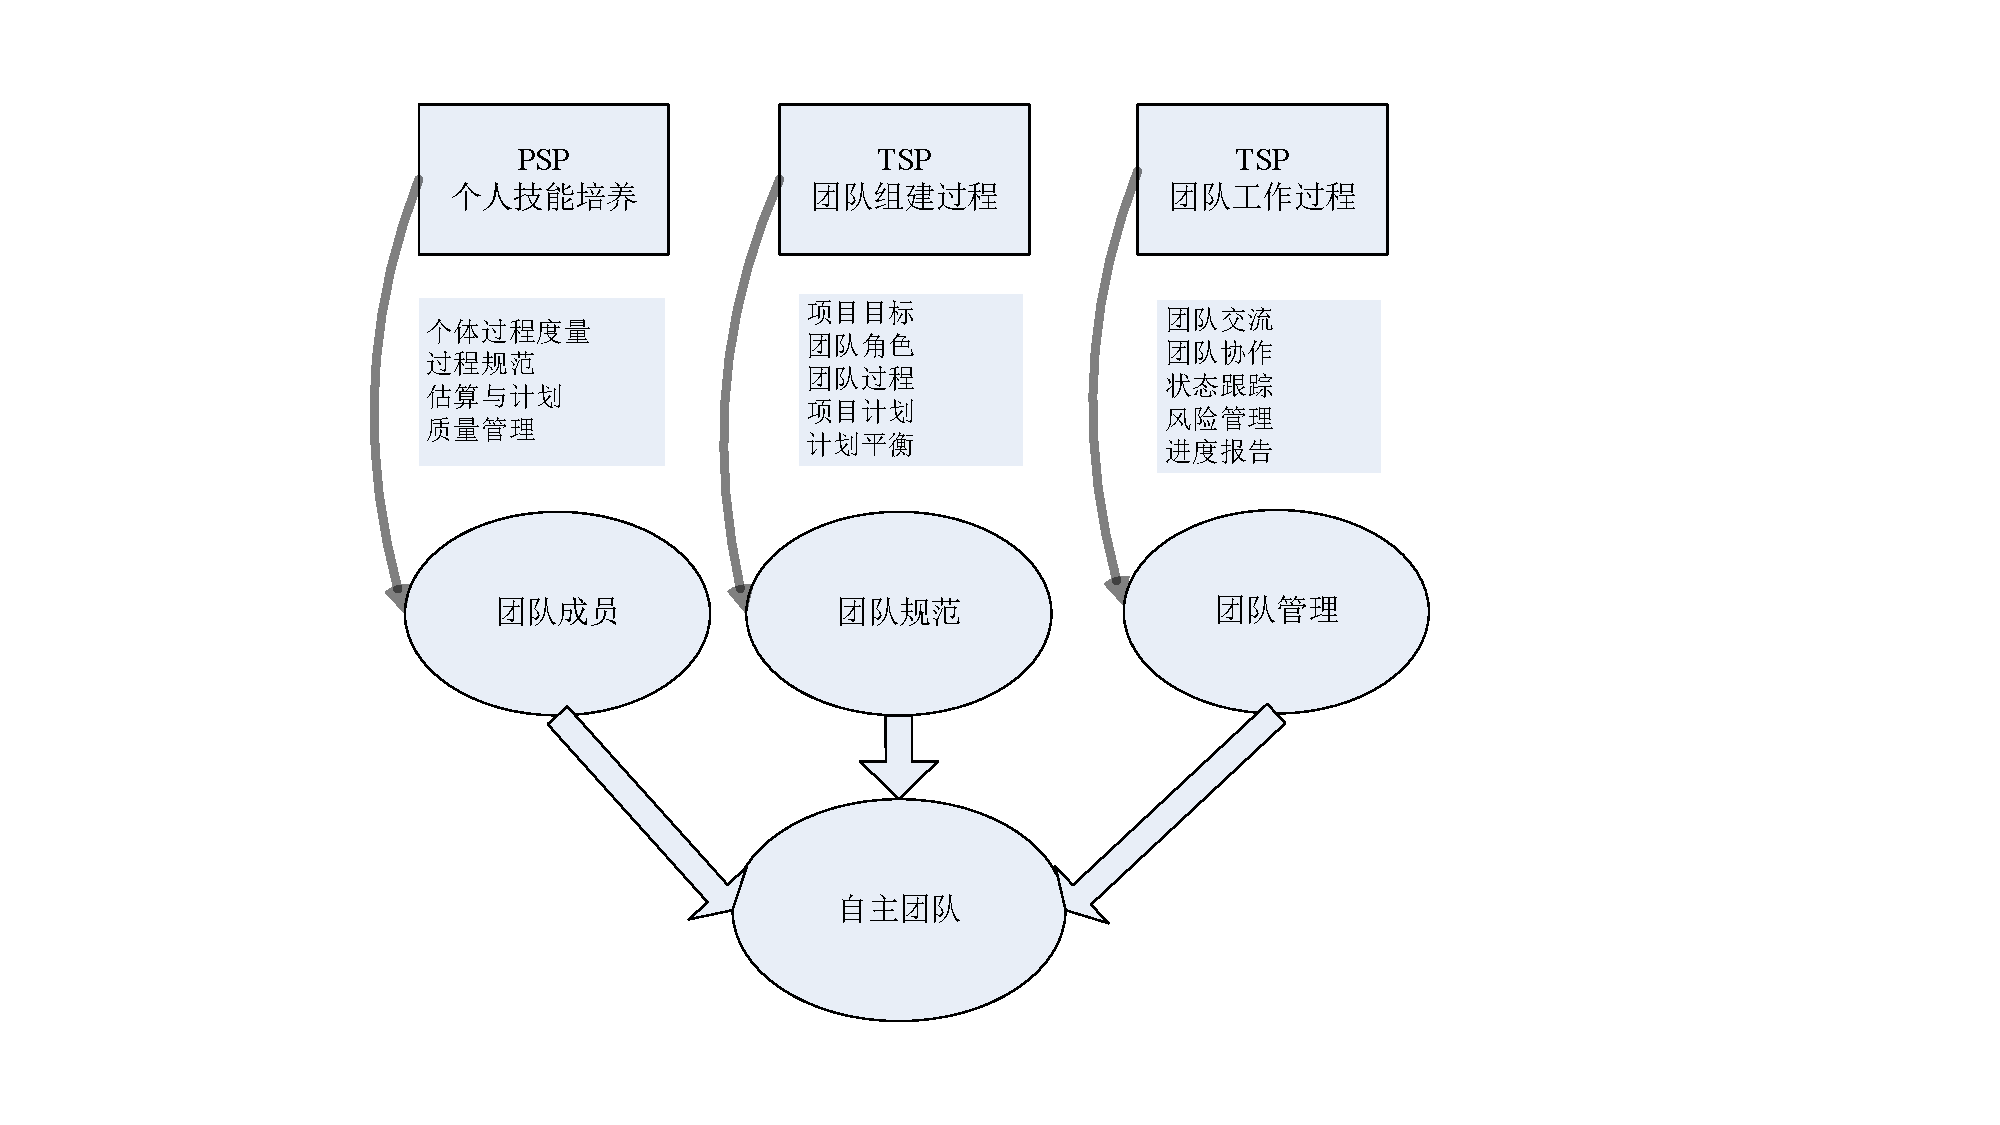
\includegraphics[width=0.6\textwidth]{images/PSP.pdf}
    \vspace{-1em}
\end{figure}
\vspace{-1em}
\end{problem}

\begin{problem}
自主团队有哪些特点?为什么说这样的团队可以满足软件开发对团队的要求?

自主团队特点如上

软件开发一种智力活动,开发者是智力劳动者,而对于智力劳动者而言,管理的第一准则就是智力劳动者不能被管理,只能实现自我管理:
\vspace{-0.8em}
\begin{multicols}{2}
    \begin{itemize}
        \item 处理和讨论非常抽象的概念
        \item 把不同的部分整合成一个可以工作的正确的系统
        \item 全身心地参与
        \item 努力做出卓越的工作
    \end{itemize}
\end{multicols}
\vspace{-1em}
\end{problem}

\begin{problem}
请结合软件开发的特点介绍软件项目管理中自主型团队的必要性以及自主团队应该具备的特征?

软件开发是一项既复杂又富有创造性的知识工作

软件开发是一种智力劳动:处理和讨论极其抽象的概念、把不同的部分(不可见)整合成一个可以工作的系统

自主团队具备如下的特点:
\vspace{-0.8em}
\begin{multicols}{2}
    \begin{itemize}
        \item 自行定义项目的目标
        \item 自行决定团队组成形式以及成员的角色
        \item 自行决定项目的开发策略
        \item 自行定义项目的开发过程
        \item 自行制定项目的开发计划
        \item 自行度量、管理和控制项目工作
    \end{itemize}
\end{multicols}
\vspace{-1em}
\end{problem}

\begin{problem}
马斯洛的“人的需求层次理论”描述的需求层次有哪几个?这样分层对软件开发有什么启发?
\end{problem}

\subsection{TSP的典型角色}
\vspace{-0.5em}
\begin{spacing}{1.2}
    \centering
    \begin{longtable}{|m{1.5cm}<{\centering}|m{4.2cm}|m{4.2cm}|m{4.2cm}|}
        \hline
        \textbf{角色} & \multicolumn{1}{c|}{\textbf{介绍}} & \multicolumn{1}{c|}{\textbf{典型技能}} & \multicolumn{1}{c|}{\textbf{工作内容}} \\ \hline
        \textbf{项目组长} & 
        项目组长的目标和衡量指标
        \begin{itemize}[leftmargin=1.3em]
            \item 建设和维持高效率的团队
            \item 激励团队成员积极工作
            \item 合理处理团队成员的问题
            \item 向管理层提供项目进度相关的完整信息
            \item 充当合格的会议组织者和协调者
            \vspace{-1.3em}
        \end{itemize} &
        \vspace{-1.1em}
        \begin{itemize}[leftmargin=1.3em]
            \item 你是天生的领导者
            \item 你有能力识别问题的关键并且做出客观的决策
            \item 你不介意偶尔充当“恶人”
            \item 你尊敬你的团队成员
            \vspace{-1.3em}
        \end{itemize} &
        \vspace{-1.1em}
        \begin{enumerate}[label=\arabic*.,leftmargin=1.5em]
            \item 激励团队成员努力工作
            \item 主持项目周例会
            \item 每周汇报项目状态
            \item 分配工作任务
            \item 维护项目资料
            \item 组织项目总结
            \vspace{-1.3em}
        \end{enumerate} \\ \hline
        \textbf{计划经理} & 
        \vspace{-1.1em}
        \begin{itemize}[leftmargin=1.3em]
            \item 开发完整的、准确的团队计划和个人计划
            \item 每周准确的报告项目小组状态
            \vspace{-1.3em}
        \end{itemize} &
        \vspace{-1.1em}
        \begin{itemize}[leftmargin=1.3em]
            \item 最为重要的一点是,你做事有条理和逻辑
            \item 你对于过程数据非常感兴趣,期待通过每周输入的数据来了解项目当前状况
            \item 你认为计划非常重要,也愿意要求团队成员跟踪和度量他们的工作
            \vspace{-1.3em}
        \end{itemize} &
        \vspace{-1.1em}
        \begin{enumerate}[label=\arabic*.,leftmargin=1.5em]
            \item 带领项目小组开发项目计划
            \item 带领项目小组平衡计划
            \item 跟踪项目进度
            \item 参与项目总结
            \vspace{-1.3em}
        \end{enumerate} \\ \hline
        \textbf{开发经理} & 
        \vspace{-1.1em}
        \begin{itemize}[leftmargin=1.3em]
            \item 开发优秀的软件产品
            \item 充分利用团队成员的技能
            \vspace{-1.3em}
        \end{itemize} &
        \vspace{-1.1em}
        \begin{itemize}[leftmargin=1.3em]
            \item 你喜欢创造事物
            \item 你愿意成为软件工程师,并且喜欢带领团队开展设计和开发工作
            \item 你具备足够的背景可以胜任设计师的工作,并且可以领导设计团队开展工作
            \item 你熟悉主流的设计工具
            \item 你愿意倾听和接受其他人的设计思想
            \vspace{-1.3em}
        \end{itemize} &
        带领团队
        \vspace{0.2em}
        \begin{enumerate}[label=\arabic*.,leftmargin=2.1em]
            \item 制定开发策略
            \item 开展产品规模估算和所需时间资源的估算
            \item 开发需求规格说明
            \item 开发高层设计
            \item 开发设计规格说明
            \item 实现软件产品
            \item 开展集成测试和系统测试
            \item 开发用户支持文档
        \end{enumerate}
        \vspace{0.3em}
        \begin{enumerate}[label=9.,leftmargin=1.5em]
            \item 参与项目总结
            \vspace{-1.3em}
        \end{enumerate} \\ \hline
        \textbf{质量经理} & 
        \vspace{-1.1em}
        \begin{itemize}[leftmargin=1.3em]
            \item 项目团队严格按照质量计划开展工作,开发出高质量的软件产品
            \item 所有的小组评审工作都正常开展,并且都形成了评审报告
            \vspace{-1.3em}
        \end{itemize} &
        \vspace{-1.1em}
        \begin{itemize}[leftmargin=1.3em]
            \item 你关注软件产品的质量
            \item 你有评审方面的经验,熟悉各种评审方法
            \item 你有协调组织有效评审的能力
            \vspace{-1.3em}
        \end{itemize} &
        \vspace{-1.1em}
        \begin{enumerate}[label=\arabic*.,leftmargin=1.5em]
            \item 带领团队开发和跟踪质量计划
            \item 向项目组长警示质量问题
            \item 软件产品提交配置管理之前,对其进行评审,以消除质量问题
            \item 项目小组评审的组织者和协调者
            \item 参与项目总结
            \vspace{-1.3em}
        \end{enumerate} \\ \hline
        \textbf{过程经理} & 
        \vspace{-1.1em}
        \begin{itemize}[leftmargin=1.3em]
            \item 所有团队成员准确的记录、报告和跟踪过程数据
            \item 所有的团队会议都有相应会议记录
            \vspace{-1.3em}
        \end{itemize} &
        \vspace{-1.1em}
        \begin{itemize}[leftmargin=1.3em]
            \item 你对过程定义、过程度量非常感兴趣
            \item 你对过程改进非常感兴趣
            \vspace{-1.3em}
        \end{itemize} &
        \vspace{-1.1em}
        \begin{enumerate}[label=\arabic*.,leftmargin=1.5em]
            \item 带领团队定义和记录开发过程并支持过程改进
            \item 建立维护团队开发标准
            \item 记录维护项目会议记录
            \item 参与项目总结
            \vspace{-1.3em}
        \end{enumerate} \\ \hline
        \textbf{支持经理} & 
        \vspace{-1.1em}
        \begin{itemize}[leftmargin=1.3em]
            \item 项目小组在整个开发过程中都有合适的工具和环境
            \item 对于基线产品,不存在非授权的变更
            \item 项目小组的风险和问题得到跟踪
            \item 项目小组在开发过程中满足复用目标
            \vspace{-1.3em}
        \end{itemize} &
        \vspace{-1.1em}
        \begin{itemize}[leftmargin=1.3em]
            \item 你对于各种开发工具很感兴趣,熟悉各类工具的适用场合
            \item 你对版本控制工具很熟悉,也熟悉配置管理流程
            \item 对于本项目所有工具而言,你都是专家
            \vspace{-1.3em}
        \end{itemize} &
        \vspace{-1.1em}
        \begin{enumerate}[label=\arabic*.,leftmargin=1.5em]
            \item 带领团队识别开发过程中所需各类工具和设施
            \item 主持配置管理委员会,管理配置管理系统
            \item 维护软件项目的词汇表
            \item 维护项目风险和问题跟踪系统
            \item 支持软件开发过程中复用策略的应用
            \item 参与项目总结
            \vspace{-1.3em}
        \end{enumerate}\\ \hline
        \textbf{开发人员} & \multicolumn{1}{c|}{—} & \multicolumn{1}{c|}{—} & \multicolumn{1}{c|}{—} \\ \hline
    \end{longtable}
\end{spacing}
\vspace{-5em}


\begin{problem}
TSP项目经理、过程经理、计划经理的工作内容、项目总结角度
\end{problem}

\begin{problem}
	下列描述当中,属于过程经理的工作内容有哪些?
	\uline{AC}    
    \vspace{-0.8em}
    \begin{multicols}{2}
        \begin{enumerate}[label=\Alph*.]
            \item 建立团队的开发标准
            \item 主持项目周例会
            \item 记录周例会的会议记录
            \item 制定开发计划
        \end{enumerate}
    \end{multicols}
    \vspace{-1em}
\end{problem}